%% BranchMorphoGen User Manual -- paper-format technical manual
%% Build:  cd docs/manual && latexmk -pdf BranchMorphoGen_UserManual.tex
\documentclass[11pt,a4paper]{article}

\usepackage[T1]{fontenc}
\usepackage[utf8]{inputenc}
\usepackage{lmodern}
\usepackage{microtype}
\usepackage[margin=2.3cm]{geometry}
\usepackage{amsmath,amssymb,bm}
\usepackage{graphicx}
\usepackage{booktabs,longtable,tabularx,array}
\usepackage{algorithm}
\usepackage[noend]{algpseudocode}
\usepackage[dvipsnames]{xcolor}
\usepackage{tikz}
\usetikzlibrary{arrows.meta,positioning,fit,calc,shapes.geometric}
\usepackage{listings}
\usepackage[font=small,labelfont=bf,margin=0.5cm]{caption}
\usepackage[numbers,sort&compress]{natbib}
\usepackage{fancyhdr}
\usepackage{enumitem}
\usepackage[section]{placeins}
\renewcommand{\topfraction}{0.92}
\renewcommand{\bottomfraction}{0.8}
\renewcommand{\textfraction}{0.06}
\renewcommand{\floatpagefraction}{0.75}
\setcounter{topnumber}{3}\setcounter{totalnumber}{5}
\usepackage[colorlinks=true,linkcolor=MidnightBlue,citecolor=MidnightBlue,urlcolor=MidnightBlue]{hyperref}

\graphicspath{{figures/}{../}}
\setlist{itemsep=2pt,topsep=4pt}
\setlength{\parskip}{3pt}

\lstset{basicstyle=\ttfamily\small,columns=fullflexible,keepspaces=true,
        frame=single,rulecolor=\color{black!25},backgroundcolor=\color{black!3},
        breaklines=true,xleftmargin=4pt,xrightmargin=4pt,aboveskip=6pt,belowskip=6pt}

\usepackage[htt]{hyphenat}
\newcommand{\code}[1]{\texttt{#1}}
\setlength{\emergencystretch}{3em}
\sloppy
\newcommand{\vect}[1]{\bm{#1}}
\newcommand{\dd}{\mathrm{d}}
\algrenewcommand\algorithmicrequire{\textbf{Input:}}
\algrenewcommand\algorithmicensure{\textbf{Output:}}

\pagestyle{fancy}
\fancyhf{}
\fancyhead[L]{\small BranchMorphoGen User Manual}
\fancyhead[R]{\small v1.0.0}
\fancyfoot[C]{\small\thepage}
\renewcommand{\headrulewidth}{0.4pt}

\title{\vspace{-1.2cm}
  \includegraphics[width=2.4cm]{../BranchMorphoGen-Logo2.png}\\[0.4cm]
  \textbf{BranchMorphoGen: a generalized framework to simulate\\ branching morphogenesis}\\[0.25cm]
  \large User manual, model physics and algorithms}
\author{Sabyasachi Sutradhar \and Sonal Shree \and Jonathon Howard\\[2pt]
  \small Howard Lab, Department of Molecular Biophysics and Biochemistry, Yale University}
\date{\small Software version 1.0.0 \quad$\cdot$\quad Manual compiled \today}

\begin{document}
\maketitle
\thispagestyle{empty}

\begin{abstract}
\noindent
The shape of a neuron sets its connectivity and how it processes signals. Many molecules are known to change neuronal shape, but how their activity produces a branched tree is still poorly understood. \textsc{BranchMorphoGen} is a fast, flexible, agent-based C++ simulator that grows branched morphologies from a few local rules measured in living cells:
\begin{itemize}
  \item stochastic, multi-state tip elongation;
  \item \emph{de novo} branching by lateral branching or tip bifurcation;
  \item contact-based self-avoidance;
  \item diameter scaling with the supported subtree;
  \item elastic straightening of branches.
\end{itemize}
It reproduces the measured development of \emph{Drosophila} class~IV dendritic arborization neurons. It also produces Purkinje cells, starburst amacrine cells, fungal mycelia and tree-like shapes.

This manual covers both the science and the software. For each module, Section~\ref{sec:model} gives the physical model, the equations it solves, and the algorithm and data structures used to implement it, with reference to the source files. Section~\ref{sec:usage} covers installation, the input file, every parameter and the output files. Section~\ref{sec:gui} describes the browser-based graphical interface and how it was built.
\end{abstract}

\tableofcontents
\newpage

%=====================================================================
\section{Introduction}
%=====================================================================
Branched networks occur at very different length and time scales: river basins, trees, fungal hyphae, lungs, kidneys, the vasculature and neurons~\cite{Hannezo2017,Uar2021}. In neurons the dendritic arbor is the substrate for synaptic input, so its geometry directly limits what the cell can compute. Many molecular factors that change dendrite shape have been identified. The mechanistic link from molecular activity to the emergent shape of a whole tree, however, is not yet understood.

Computational models are a natural way to bridge these scales. Earlier generative models include the following:
\begin{itemize}
  \item optimal-wiring approaches~\cite{Cuntz2010};
  \item phenomenological growth-cone models such as NETMORPH~\cite{Koene2009};
  \item system-specific stochastic models~\cite{Palavalli2021,Castro2020,Ganguly2016};
  \item continuum theories of branching~\cite{Hannezo2017,Uar2021}.
\end{itemize}
These models are often specific to one system, need a predetermined template, or are not grounded in the measured growth dynamics of the cell.

\textsc{BranchMorphoGen} takes a different route. Every terminal branch is an \emph{agent} whose behaviour follows rules measured by time-lapse imaging~\cite{Shree2022,Ouyang2025}. The global morphology is never imposed; it \emph{emerges} from those rules. The framework is modular. Each of the five processes in Fig.~\ref{fig:modules} can be switched on, switched off or replaced through a plain-text parameter file, so the same executable produces neurons, fungi and plants. Because it is written in C++17 with collision detection that scales close to linearly, a full 120-hour class~IV neuron with $\sim$10$^6$ points runs in minutes. This makes it practical to scan high-dimensional parameter spaces.

\paragraph{Typical uses.}
\begin{enumerate}
  \item Testing mechanistic hypotheses, for example ``is contact-induced retraction sufficient to tile the body wall?''
  \item Predicting how a molecular perturbation, such as a change in tip-switching rates, changes the global architecture.
  \item Producing realistic synthetic morphologies, together with matching synthetic microscopy images, to benchmark image-analysis pipelines or train machine-learning models.
\end{enumerate}

\begin{figure}[!htbp]
  \centering
  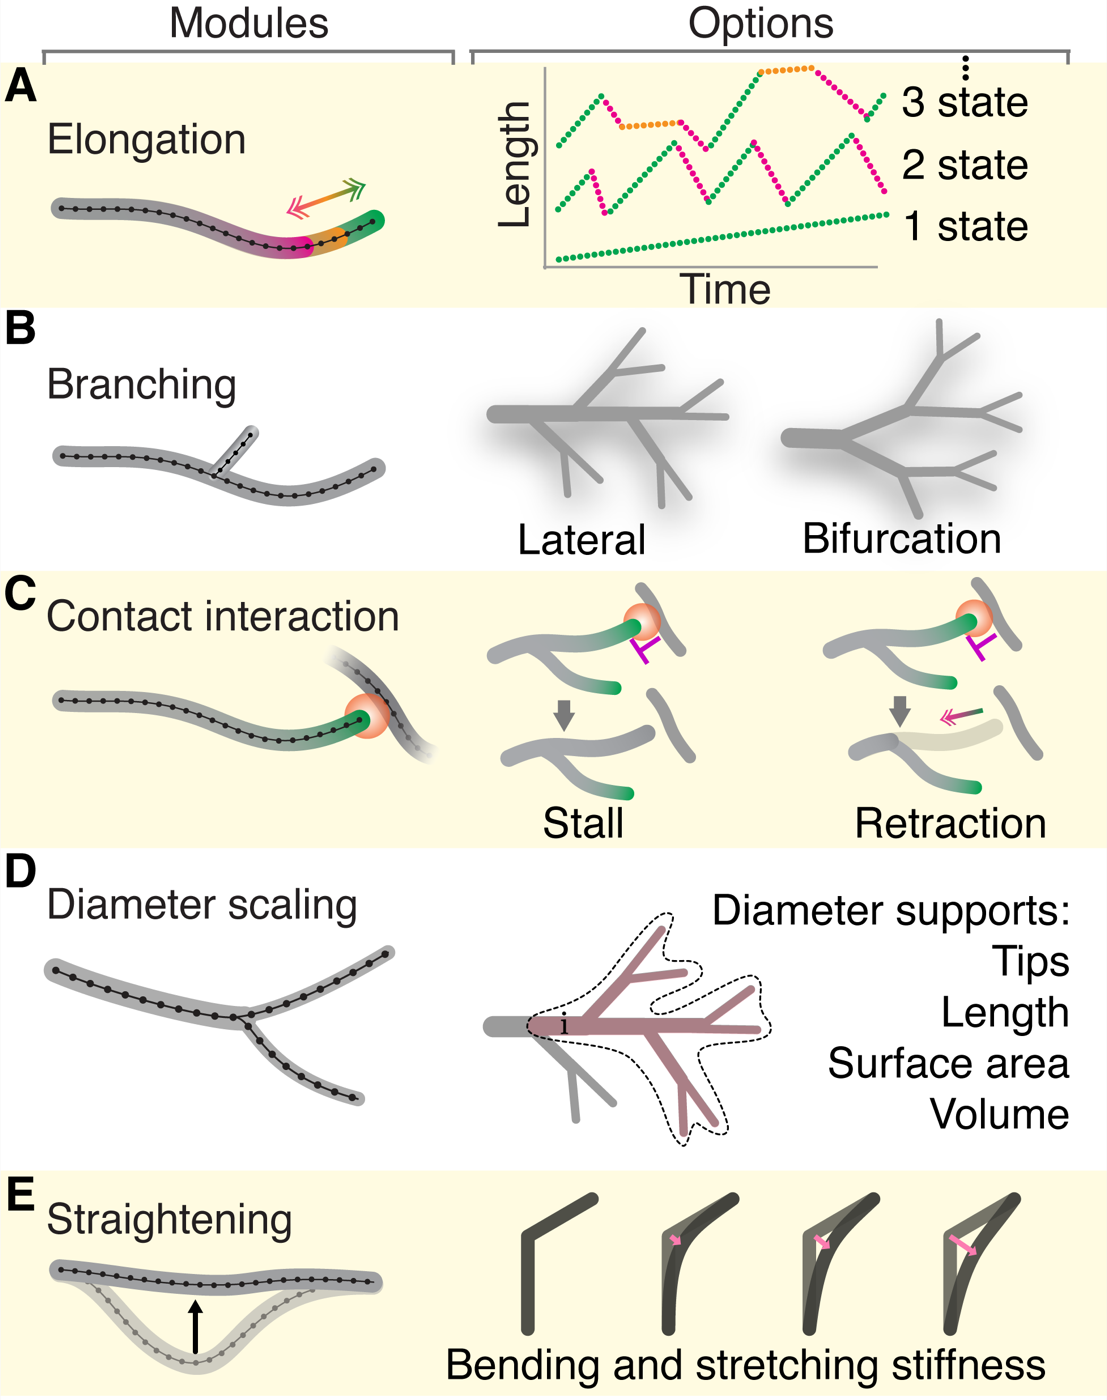
\includegraphics[width=0.78\textwidth]{fig1_modules.png}
  \caption{\textbf{The five modules of BranchMorphoGen (left) and the options available for each (right).}
  \textbf{(A)~Elongation.} A tip is a stochastic switch among $n$ states, each with its own velocity. Illustrated: one state (constant growth), two states (growth/shrinkage) and three states (growth/pause/shrinkage).
  \textbf{(B)~Branching.} New branches arise at random, either laterally along an existing branch or by bifurcation of a tip.
  \textbf{(C)~Contact interaction.} A tip that touches another branch (red halo) either stalls or retracts.
  \textbf{(D)~Diameter scaling.} The diameter of branch $i$ is set by the subtree it supports: its tips, length, surface area or volume.
  \textbf{(E)~Straightening.} Branches are elastic rods with bending and stretching stiffness, so sharp kinks relax over time.}
  \label{fig:modules}
\end{figure}

%=====================================================================
\section{Model and algorithms}\label{sec:model}
%=====================================================================

\subsection{Overview of a time step}
The simulation advances the whole tree with a fixed time step $\Delta t$ (\code{Dt}) from $T_i$ (\code{Time\_Start}) to $T_f$ (\code{Time\_End}). Each step applies the modules in a fixed order (Algorithm~\ref{alg:step}, \code{src/Simulation.cpp}). The order matters:
\begin{itemize}
  \item Growth and branching act on the current geometry.
  \item Deleted branches are removed before the mechanics solve, so the solver always sees a valid tree.
  \item The radius is updated just before the mechanics, because the stiffnesses depend on it.
\end{itemize}

\begin{algorithm}[!htbp]
\caption{One simulation step (\code{Simulation::Step})}\label{alg:step}
\begin{algorithmic}[1]
\Require tree $\mathcal{T}$ (list of branches), step index $n$, time $t$
\State Evaluate the time-dependent parameters at $t$: velocities $\vect v(t)$, rate matrix $\mathbf K(t)$, branching rate $k_b(t)$, box $\mathcal B(t)$
\If{$n \bmod n_\text{coll}=0$} \State rebuild the broad-phase neighbour lists (Alg.~\ref{alg:neigh}) \EndIf
\ForAll{branches $b\in\mathcal T$}
   \State advance age and post-collision clock; apply termination with rate \code{TerminationRate}
   \If{$b$ is dynamic and not terminated}
      \State update the tip state by the Markov jump (Alg.~\ref{alg:state})
      \If{no state change this step} \State grow or retract the tip by $v_b\,\Delta t$ (Alg.~\ref{alg:grow}) \EndIf
   \EndIf
\EndFor
\ForAll{branches $b$ present at the start of the step}
   \State attempt lateral branching or bifurcation (Alg.~\ref{alg:branch})
\EndFor
\State remove the branches queued for deletion and repair the topology (Sec.~\ref{sec:topology})
\If{$n \bmod n_F = 0$}
   \State update all radii from subtree statistics (Alg.~\ref{alg:radius})
   \If{\code{StraightenBranches}} \State semi-implicit mechanics update over $n_F\Delta t$ (Alg.~\ref{alg:mech}) \EndIf
\EndIf
\State write the time series every unit time, and SWC/TIFF/CSV every $n_\text{SWC}$ steps
\end{algorithmic}
\end{algorithm}

\FloatBarrier
%---------------------------------------------------------------------
\subsection{Geometry and representation of the tree}
%---------------------------------------------------------------------
\begin{figure}[!htbp]
  \centering
  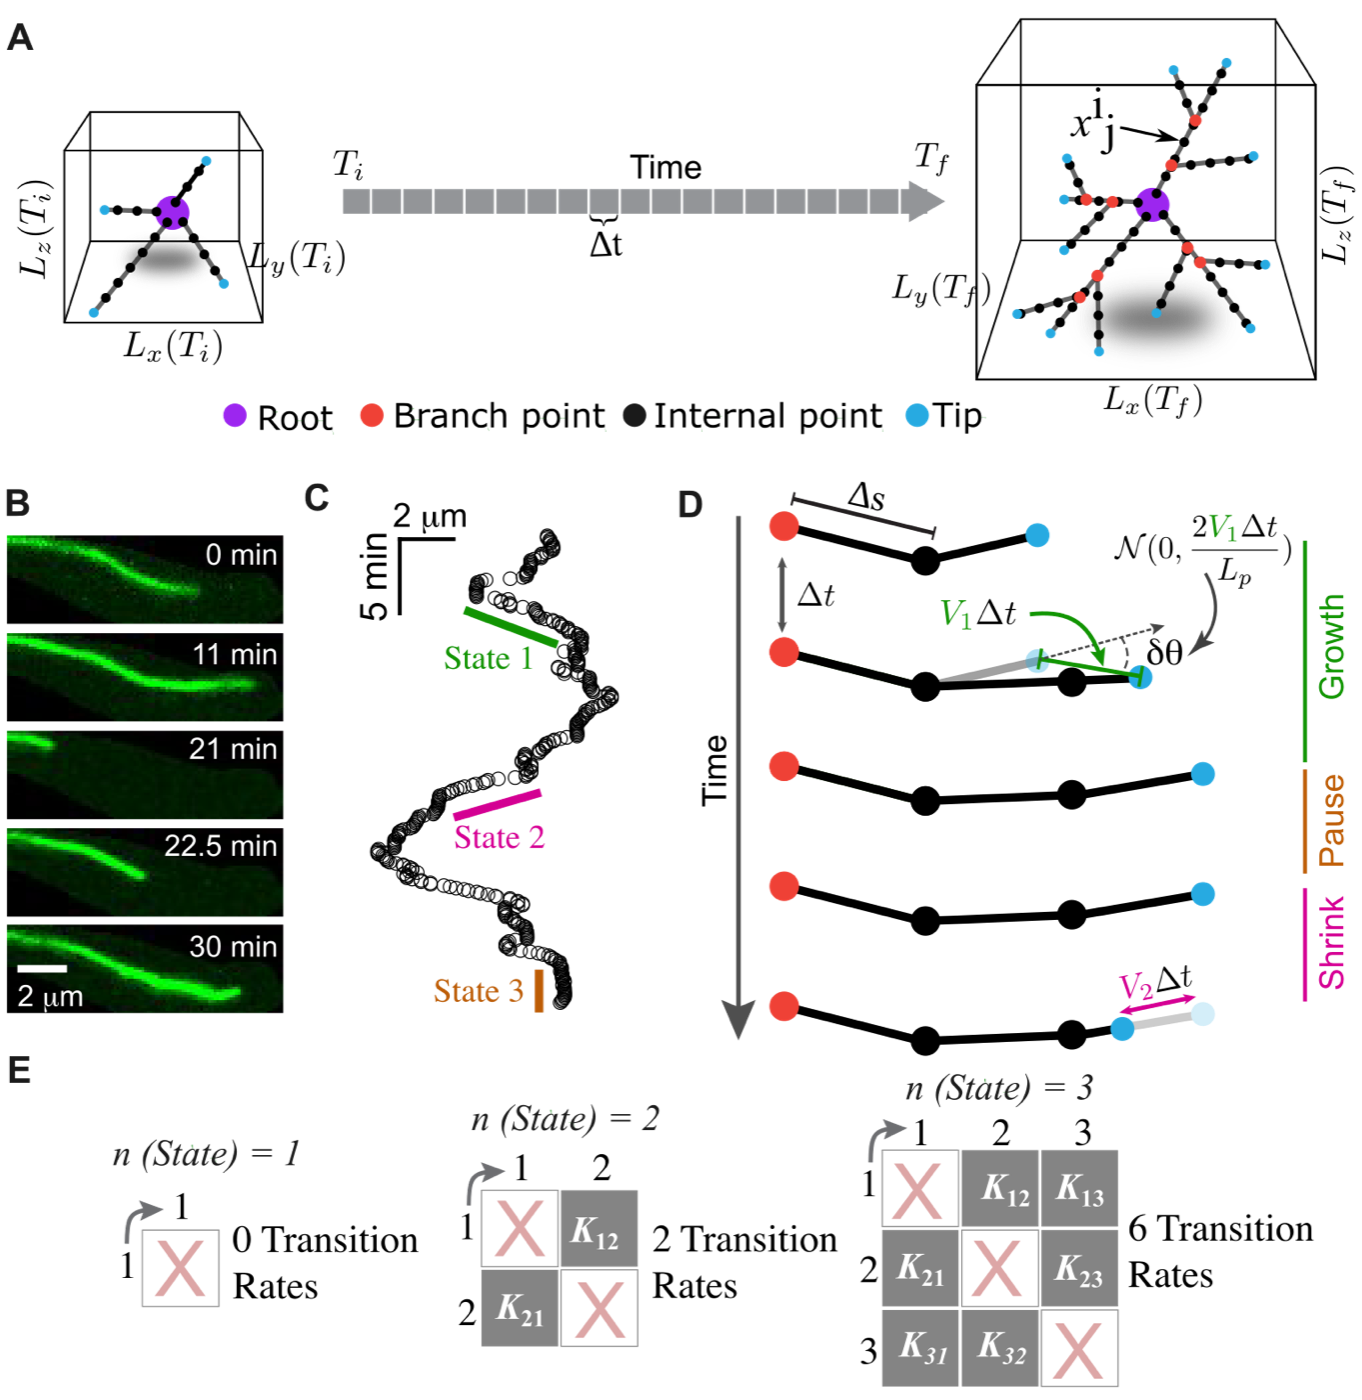
\includegraphics[width=0.86\textwidth]{fig2_tip_dynamics.png}
  \caption{\textbf{Basic set-up and elongation dynamics.}
  \textbf{(A)} The simulation box $L_{x,y,z}(t)$ can grow from $T_i$ to $T_f$. Point colours: the root (purple), branch points (orange), internal points (black) and tips (blue). $\vect x^i_j$ is point $j$ of branch $i$.
  \textbf{(B)} Time-lapse images of a class~IV dendrite tip that grows, pauses and shrinks.
  \textbf{(C)} Tracked tip length against time. Segments of constant slope define states 1--3.
  \textbf{(D)} What one time step does. A growing tip advances by $V_1\Delta t$. Its direction is perturbed by $\delta\theta\sim\mathcal N(0,2V_1\Delta t/L_p)$. A paused tip stays put, and a shrinking tip retracts by $V_2\Delta t$. Points are spaced $\Delta s$ apart.
  \textbf{(E)} An $n$-state model needs the $n(n-1)$ off-diagonal entries of the transition-rate matrix.}
  \label{fig:tip}
\end{figure}

The arbor is a rooted binary tree of \emph{branches} (Fig.~\ref{fig:tip}A). A branch $i$ is an ordered list of points $\{\vect x^i_0,\dots,\vect x^i_{N_i}\}$, spaced $\Delta s$ (\code{BranchInterval}) apart along its centreline. It stores:
\begin{itemize}
  \item a base point, which is the last point of its parent or the root;
  \item the indices of its parent, sibling and two children;
  \item a radius $r_i$, a tip state $s_i$, a velocity $v_i$ and its age;
  \item flags: \code{Dynamic} (it has a free tip), \code{Initial} (it is a primary branch leaving the soma), \code{Collision}, \code{Termination};
  \item an axis-aligned bounding box (AABB) and a neighbour list (Sec.~\ref{sec:collision}).
\end{itemize}

Point types follow from the number of children:
\begin{itemize}
  \item a point with one child is an \emph{internal} point;
  \item a point with two children is a \emph{branch point};
  \item a point with none is a \emph{tip}.
\end{itemize}
Only terminal (dynamic) branches change state and length. Internal branches move only passively, through the mechanics.

Branches are stored in one contiguous \code{std::vector}. Parent and child links are integer indices, not pointers. This keeps the data cache-friendly and makes the arrays simple to compact after deletions.

\paragraph{Boundary.}
The domain is a box $\mathcal B(t)=[x_-,x_+]\times[y_-,y_+]\times[z_-,z_+]$. Its limits are given as tables in time (\code{LimitsX/Y/Z}) and interpolated linearly, so the box can expand as the larva grows. A \emph{soft} margin of width $\ell_s$ (\code{Boundary\_SoftLength}) lets tips cross the wall slightly before they are pushed back (Sec.~\ref{sec:boundary}).

\paragraph{Initial condition.}
There are two ways to start:
\begin{itemize}
  \item \textbf{From scratch.} $N_0$ primary branches of length \code{InitialLength} leave the soma, which has radius $R_s$ (\code{RadiusSoma}) and sits at \code{Root}. $N_0$ may be a range \code{a-b}, sampled once per sample. Their orientation is set by \code{InitialAngle} (in-plane) and \code{InitialAngleWithZ} (tilt from the $z$-axis).
  \item \textbf{From reconstructed SWC files} (\code{src/ReadSWC.cpp}). The file is parsed into the same branch structure. Given a folder, each \code{.swc} file becomes its own sample.
\end{itemize}

\FloatBarrier
%---------------------------------------------------------------------
\subsection{Tip dynamics: a multi-state stochastic switch}\label{sec:tip}
%---------------------------------------------------------------------
\paragraph{Physics.}
Dendrite tips of class~IV neurons show \emph{dynamic instability}, like microtubules. They switch at random between growing, paused and shrinking states, each with a characteristic speed (Fig.~\ref{fig:tip}B--C)~\cite{Shree2022}. We model each tip as a continuous-time Markov chain over $n$ discrete states $\{1,\dots,n\}$ (\code{States}) with velocities $v_1,\dots,v_n$ (\code{StateVelocity}). Switching rates form the matrix $\mathbf K=(K_{ij})$ (\code{TransitionRates}), where $K_{ij}$ is the rate of switching $i\to j$ and $K_{ii}=0$. The occupation probabilities $p_i(t)$ obey the master equation
\begin{equation}
  \frac{\dd p_i}{\dd t}=\sum_{j\neq i}\left(K_{ji}\,p_j-K_{ij}\,p_i\right),
\end{equation}
and the tip length $L$ obeys $\dot L=v_{s(t)}$. Over long times the tip performs a biased random walk. Its drift is the state-averaged velocity
\begin{equation}
  \bar v=\sum_i \pi_i v_i ,\qquad \text{with}\quad \sum_{j\ne i}\pi_j K_{ji}=\pi_i\sum_{j\ne i}K_{ij},
\end{equation}
where $\pi$ is the stationary distribution. Its effective diffusion coefficient is set by the velocity differences and the switching times.

When $\bar v<0$, an isolated tip has a finite, exponentially distributed length (bounded growth). When $\bar v>0$ it grows without bound. This is the same transition as for dynamic microtubules~\cite{Dogterom1993}, and it is why the simple local rules can produce both sparse and dense arbors~\cite{Shree2022,Ouyang2025}. $\vect v$ and $\mathbf K$ can depend on time (Sec.~\ref{sec:timedep}), which captures the change in dynamics over larval development (Table~\ref{tab:classiv}).

\paragraph{Algorithm.}
At every step, each dynamic tip undergoes at most one jump. With $k_\text{tot}=\sum_{j\neq s}K_{sj}$, the probability of leaving state $s$ during $\Delta t$ is $1-e^{-k_\text{tot}\Delta t}$, which is exact for constant rates. The target state is then picked in proportion to the rates, as in the direct method of Gillespie~\cite{Gillespie1977} (Algorithm~\ref{alg:state}, \code{BranchGrowth::updateState}).

The fixed-step scheme is accurate when $k_\text{tot}\Delta t\ll 1$. For the class~IV rates ($k_\text{tot}\lesssim 2\,\text{min}^{-1}$) and $\Delta t=0.025$\,min, the probability of two jumps in one step is below $10^{-3}$.

A one-state model skips the jump entirely and gives constant growth. While a branch is in contact (Sec.~\ref{sec:collision}), the same routine uses the collision state set (\code{Collision\_States}, \code{Collision\_StateVelocity}, \code{Collision\_TransitionRates}).

\begin{algorithm}[!htbp]
\caption{Markov state update of a tip (\code{BranchGrowth::updateState})}\label{alg:state}
\begin{algorithmic}[1]
\Require branch $b$ in state $s$; rate matrix $\mathbf K$ ($\mathbf K^\text{coll}$ if $b$ is in contact); velocities $\vect v$
\State $k_\text{tot}\gets\sum_{j\ne s}K_{sj}$
\State draw $u_1\sim\mathcal U(0,1)$; \textbf{if} $u_1\ge 1-e^{-k_\text{tot}\Delta t}$ \textbf{then return} \Comment{no jump}
\State draw $u_2\sim\mathcal U(0,1)$; find the smallest $j\neq s$ with $\sum_{j'\le j,\,j'\ne s}K_{sj'}/k_\text{tot}>u_2$
\State $s_b\gets j$, \; $v_b\gets v_j$
\If{$b$ is primary and $L_b<R_s$} reset $b$ to the growing state \Comment{keep tips out of the soma} \EndIf
\end{algorithmic}
\end{algorithm}

\FloatBarrier
%---------------------------------------------------------------------
\subsection{Elongation and retraction with directional persistence}
%---------------------------------------------------------------------
\paragraph{Physics.}
Growing tips do not move in perfectly straight lines. We treat the growth direction as a persistent random walk on the unit sphere, like a worm-like chain. The tangent $\hat{\vect t}$ receives a random rotation whose variance grows linearly with the added length $\Delta\ell=v\Delta t$:
\begin{equation}
  \hat{\vect t}' = \frac{\hat{\vect t}+\vect\xi_\perp}{\lVert\hat{\vect t}+\vect\xi_\perp\rVert},\qquad
  \xi_\alpha\sim\mathcal N\!\left(0,\;\sigma^2\right),\quad \sigma^2=\frac{2\,\Delta\ell}{L_p},
\end{equation}
where $\vect\xi_\perp$ is the component of a Gaussian vector perpendicular to the current direction, and $L_p$ is \code{PersistanceLength}.

In two dimensions the turning angle has variance $\langle\delta\theta^2\rangle=\sigma^2$. Hence $\langle\cos\delta\theta\rangle\simeq e^{-\Delta\ell/L_p}$, and the tangent correlation decays as $\langle\hat{\vect t}(s)\cdot\hat{\vect t}(0)\rangle=e^{-s/L_p}$, so $L_p$ is exactly the persistence length of the growth path. In three dimensions there are two perpendicular components, so the decay length of the tangent correlation is $L_p/2$. Setting $L_p=\infty$ (\code{inf}) gives straight growth (Fig.~\ref{fig:branching}C).

\paragraph{Algorithm.}
Growth and retraction both edit the point list near the tip (Algorithm~\ref{alg:grow}, \code{BranchGrowth::\allowbreak addLengthToTip} and \code{retractLengthFromTip}). Every point is kept at spacing $\Delta s$ except the last segment, which holds the remainder.
\begin{itemize}
  \item \textbf{Growth.} Before growing, the tip is checked for contact with other branches, the boundary and the soma. If any contact is found, the tip enters the collision state instead of advancing.
  \item \textbf{Retraction.} The tip walks back along the contour to the new length $L-|\Delta\ell|$ and is interpolated there. If the branch would become shorter than its attachment zone, it is removed. The attachment zone is $R_s$ for primary branches and $r_\text{parent}+\Delta s$ otherwise. Exceptions:
  \begin{itemize}
    \item primary branches always regrow;
    \item other branches regrow with probability \code{RebranchingProb}.
  \end{itemize}
\end{itemize}

\begin{algorithm}[!htbp]
\caption{Tip elongation and retraction (\code{BranchGrowth::updateGrowth})}\label{alg:grow}
\begin{algorithmic}[1]
\Require branch $b$ with points $\vect x_0..\vect x_N$, velocity $v_b$
\State $\Delta\ell\gets v_b\Delta t$
\If{$\Delta\ell>0$}
  \If{tip contacts a branch, the boundary or the soma} \State enter collision state: $s_b\gets\arg\min_j v^\text{coll}_j$, start the post-collision clock; \textbf{return}\EndIf
  \State $\hat{\vect t}\gets(\vect x_N-\vect x_{N-1})/\lVert\cdot\rVert$; perturb to $\hat{\vect t}'$ with variance $2\Delta\ell/L_p$
  \State remove $\vect x_N$; starting from $\vect x_{N-1}$, add points along $\hat{\vect t}'$ in steps of $\min(\Delta s,\text{remaining})$ until the length $\lVert\vect x_N-\vect x_{N-1}\rVert+\Delta\ell$ is used up
\ElsIf{$\Delta\ell<0$}
  \State $L'\gets L_b-|\Delta\ell|$
  \If{$L'>R_\text{attach}$} keep the points up to arc length $L'$ and interpolate the new tip
  \ElsIf{$b$ is primary \textbf{or} $u<p_\text{rebranch}$} reset $b$ to the growing state
  \Else\ queue $b$ for deletion
  \EndIf
\EndIf
\State update the contour length, the end-to-end distance and the AABB of $b$
\end{algorithmic}
\end{algorithm}

\FloatBarrier
%---------------------------------------------------------------------
\subsection{Branching}\label{sec:branching}
%---------------------------------------------------------------------
\begin{figure}[!htbp]
  \centering
  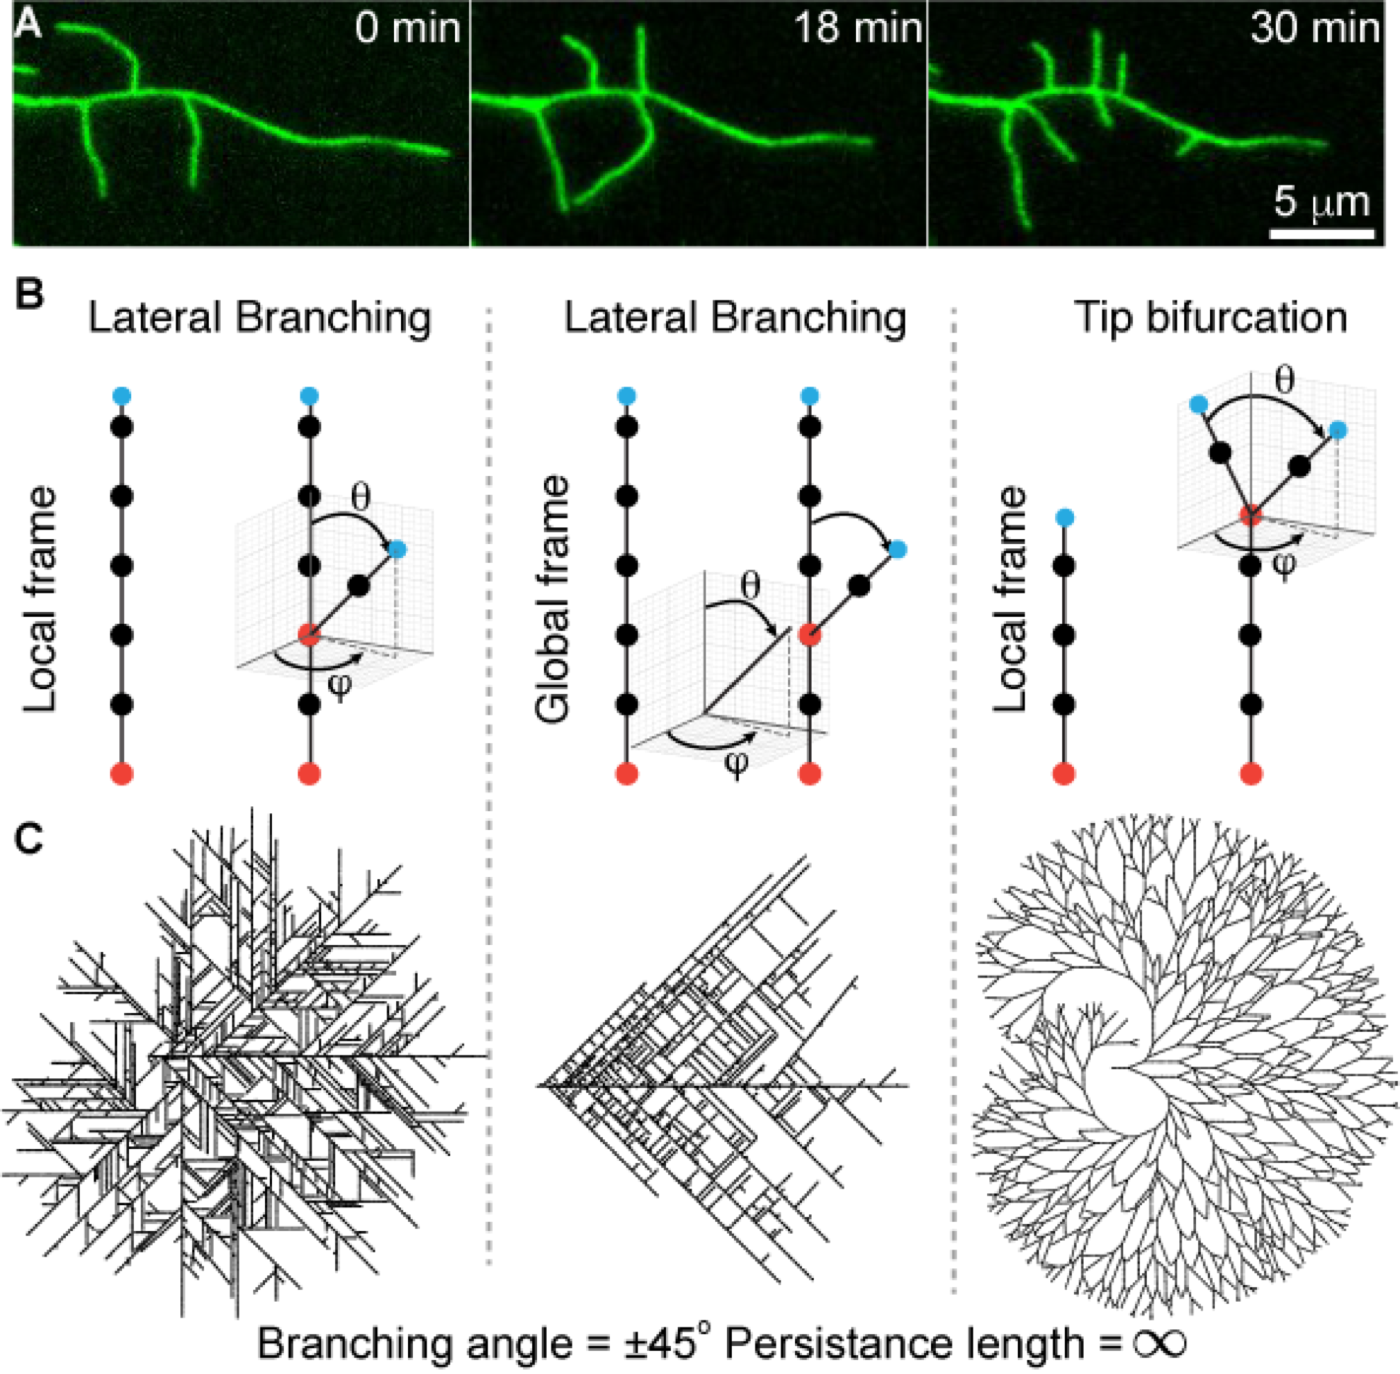
\includegraphics[width=0.78\textwidth]{fig3_branching.png}
  \caption{\textbf{Modes of branching.}
  \textbf{(A)} A new lateral branch appears and grows over 30\,min on a class~IV dendrite.
  \textbf{(B)} How new branch directions are defined. Left: lateral branching in the \emph{local} frame, with polar ($\theta$) and azimuthal ($\varphi$) angles measured from the parent's tangent at the branch point (red). Middle: lateral branching in the \emph{global} frame, with angles measured from the fixed axes. Right: tip bifurcation, where the tip splits into two daughters separated by $\theta$.
  \textbf{(C)} Trees grown with each rule, using a branching angle of $\pm45^\circ$ and $L_p=\infty$. The local frame gives an isotropic, space-filling lattice. The global frame gives strongly oriented, comb-like growth. Bifurcation gives a dichotomous, fan-shaped tree.}
  \label{fig:branching}
\end{figure}

\paragraph{Physics.}
Branch formation is a Poisson process with rate $k_b(t)$ (\code{BranchingRate}). In one step, a branch of length $L$ spawns a new branch with probability
\begin{equation}
  P_b=\begin{cases}1-e^{-k_b L\,\Delta t} & \text{length-dependent (\code{LengthDependentBranching=true})},\\[2pt]
                   1-e^{-k_b\,\Delta t} & \text{otherwise.}\end{cases}
\end{equation}
In the length-dependent case $k_b$ is a rate per unit length, so the arbor as a whole branches at rate $k_b\,L_\text{total}$, which matches measurements in class~IV neurons~\cite{Shree2022}. Because the process is random and memoryless, the model does not produce stereotyped branching programmes such as those of the lung or kidney.

\paragraph{Lateral (interstitial) branching.}
Any branch, internal or terminal, can sprout a side branch (\code{BranchSpawn::\allowbreak spawnBranch}). The following conditions apply:
\begin{itemize}
  \item \textbf{Eligibility.} The branch must be longer than $\ell_\text{th}=r_\text{parent}+r_\text{child}+2r_\text{min}+4\Delta s$, so that new branch points are not crowded at an existing junction.
  \item \textbf{Base point.} It is chosen uniformly among the interior points outside the parent and child radii, and never inside the soma.
  \item \textbf{Splitting.} The topology update splits the branch at the base point into three branches (Fig.~\ref{fig:split}):
  \begin{itemize}
    \item the proximal part stays as the parent and becomes internal;
    \item the distal part becomes a new branch that inherits the old tip state, velocity and children;
    \item the nascent branch starts in state 1 (growth) with radius $r_\text{min}$.
  \end{itemize}
  \item \textbf{Nascent growth.} The nascent branch is laid out point by point up to length \code{NascentBranchLength}$+r$. If it hits an existing branch while doing so, the event is cancelled.
\end{itemize}

\paragraph{Tip bifurcation.}
With \code{Bifurcation=true}, only dynamic tips branch (\code{BranchSpawn::\allowbreak bifurcateBranch}). The tip becomes a branch point with two nascent daughters. The opening angle $\theta\sim|\mathcal N(\bar\theta,\sigma_\theta)|$ is shared between the two daughters as $\theta_1=\theta\,\rho/(1+\rho)$ and $\theta_2=\theta/(1+\rho)$, where $\rho$ is \code{BifurcationRatio}:
\begin{itemize}
  \item $\rho=1$: symmetric Y-shape;
  \item $\rho\to0$: one daughter continues straight and the other turns, i.e.\ monopodial branching.
\end{itemize}
In \code{reflective} mode the two angles are swapped at random.

\paragraph{Branching angles.}
The new direction is given by a polar angle $\theta$ and an azimuthal angle $\varphi$. Each is drawn from $\mathcal N(\bar\theta,\sigma)$ or $\mathcal N(\bar\varphi,\sigma)$, with $\sigma$ = \code{BranchingAngleSTD}, and then handled by its mode:
\begin{description}[leftmargin=2.2cm,style=nextline]
  \item[\code{fixed}] used as drawn, so all branches leave on the same side;
  \item[\code{reflective}] mirrored with probability $1/2$ ($\varphi\to2\pi-\varphi$, $\theta\to-\theta$), giving alternating, left/right symmetric branching;
  \item[\code{uniform}] $\varphi\sim\mathcal U[0,2\pi)$, $\theta\sim\mathcal U[0,\pi)$, i.e.\ isotropic.
\end{description}
In the \code{local} frame the direction is defined about the parent tangent $\hat{\vect t}$:
\begin{itemize}
  \item in 2-D the new direction is at angle $\operatorname{atan2}(t_y,t_x)+\varphi$;
  \item in 3-D a unit vector with spherical angles $(\theta,\varphi)$ is built about $\hat{\vect z}$ and rotated so that $\hat{\vect z}\mapsto\hat{\vect t}$ (\code{Vec3::rotateZTo}).
\end{itemize}
In the \code{global} frame the direction is $(\sin\theta\cos\varphi,\sin\theta\sin\varphi,\cos\theta)$ regardless of the parent's orientation. This is how planar, oriented arbors such as Purkinje cells are produced. For class~IV neurons the measured branching angle is about $90^\circ\pm26^\circ$.

\begin{figure}[!htbp]
\centering
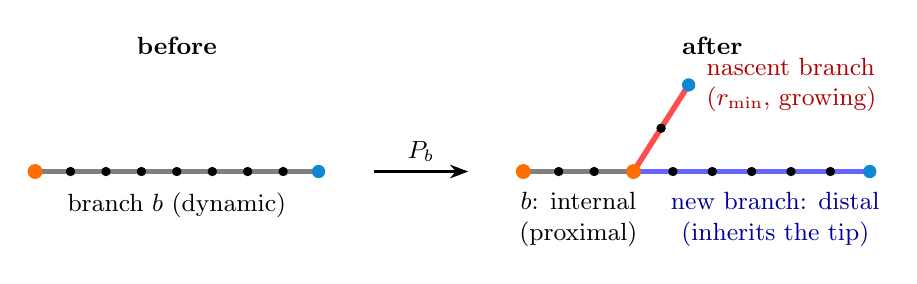
\begin{tikzpicture}[x=1cm,y=1cm, every node/.style={font=\small},
  pt/.style={circle,fill=black,inner sep=1.2pt}, tip/.style={circle,fill=cyan!70!blue,inner sep=1.7pt},
  bp/.style={circle,fill=orange!85!red,inner sep=1.9pt}]
  % before
  \node[font=\small\bfseries] at (1.8,1.6) {before};
  \draw[line width=2pt,gray] (0,0) -- (3.6,0);
  \foreach \x in {0.45,0.9,...,3.2} \node[pt] at (\x,0) {};
  \node[bp] at (0,0) {}; \node[tip] at (3.6,0) {};
  \node[below=4pt] at (1.8,0) {branch $b$ (dynamic)};
  \draw[-{Stealth},thick] (4.3,0) -- (5.5,0) node[midway,above]{$P_b$};
  % after
  \node[font=\small\bfseries] at (8.6,1.6) {after};
  \draw[line width=2pt,gray] (6.2,0) -- (7.6,0);
  \draw[line width=2pt,blue!60] (7.6,0) -- (10.6,0);
  \draw[line width=2pt,red!70] (7.6,0) -- (8.3,1.1);
  \foreach \x in {6.65,7.1} \node[pt] at (\x,0) {};
  \foreach \x in {8.1,8.6,9.1,9.6,10.1} \node[pt] at (\x,0) {};
  \node[pt] at (7.95,0.55) {};
  \node[bp] at (6.2,0) {}; \node[bp] at (7.6,0) {}; \node[tip] at (10.6,0) {}; \node[tip] at (8.3,1.1) {};
  \node[below=4pt,align=center] at (6.9,0) {$b$: internal\\(proximal)};
  \node[below=4pt,align=center,blue!60!black] at (9.4,0) {new branch: distal\\(inherits the tip)};
  \node[right=3pt,red!70!black,align=left] at (8.3,1.1) {nascent branch\\($r_\text{min}$, growing)};
\end{tikzpicture}
\caption{\textbf{Topology update for lateral branching.} The parent is split at the chosen base point. The proximal piece stays in place and becomes an internal branch. The distal piece becomes a new branch with the original tip state and children. The nascent side branch is added as its sibling. All links are integer indices into the branch array.}
\label{fig:split}
\end{figure}

\begin{algorithm}[!htbp]
\caption{Lateral branching of branch $b$ (\code{BranchSpawn::\allowbreak spawnBranch})}\label{alg:branch}
\begin{algorithmic}[1]
\If{$b$ queued for deletion, frozen after contact, terminated, or $L_b\le\ell_\text{th}$} \textbf{return} \EndIf
\State draw $u$; \textbf{if} $u\ge P_b$ \textbf{return}
\State pick base index $k$ uniformly in $[\lceil r_\text{par}/\Delta s\rceil+1,\;N-\lceil r_\text{ch}/\Delta s\rceil]$; reject if $\vect x_k$ is inside the soma
\State sample $(\theta,\varphi)$ by the angle modes; build the direction $\hat{\vect d}$ in the local or global frame
\State grow the nascent branch from $\vect x_k$ along $\hat{\vect d}$ in steps $\Delta s$; \textbf{if} it contacts a branch \textbf{return} (cancelled)
\State split $b$: proximal $\to b$ (internal), distal $\to$ new branch $b_1$, nascent $\to b_2$; set parent/sibling/child indices
\State re-point the children of the old $b$ to $b_1$; append $b_1,b_2$ and their AABBs
\end{algorithmic}
\end{algorithm}

\FloatBarrier
%---------------------------------------------------------------------
\subsection{Contact interaction and fast collision detection}\label{sec:collision}
%---------------------------------------------------------------------
\begin{figure}[!htbp]
  \centering
  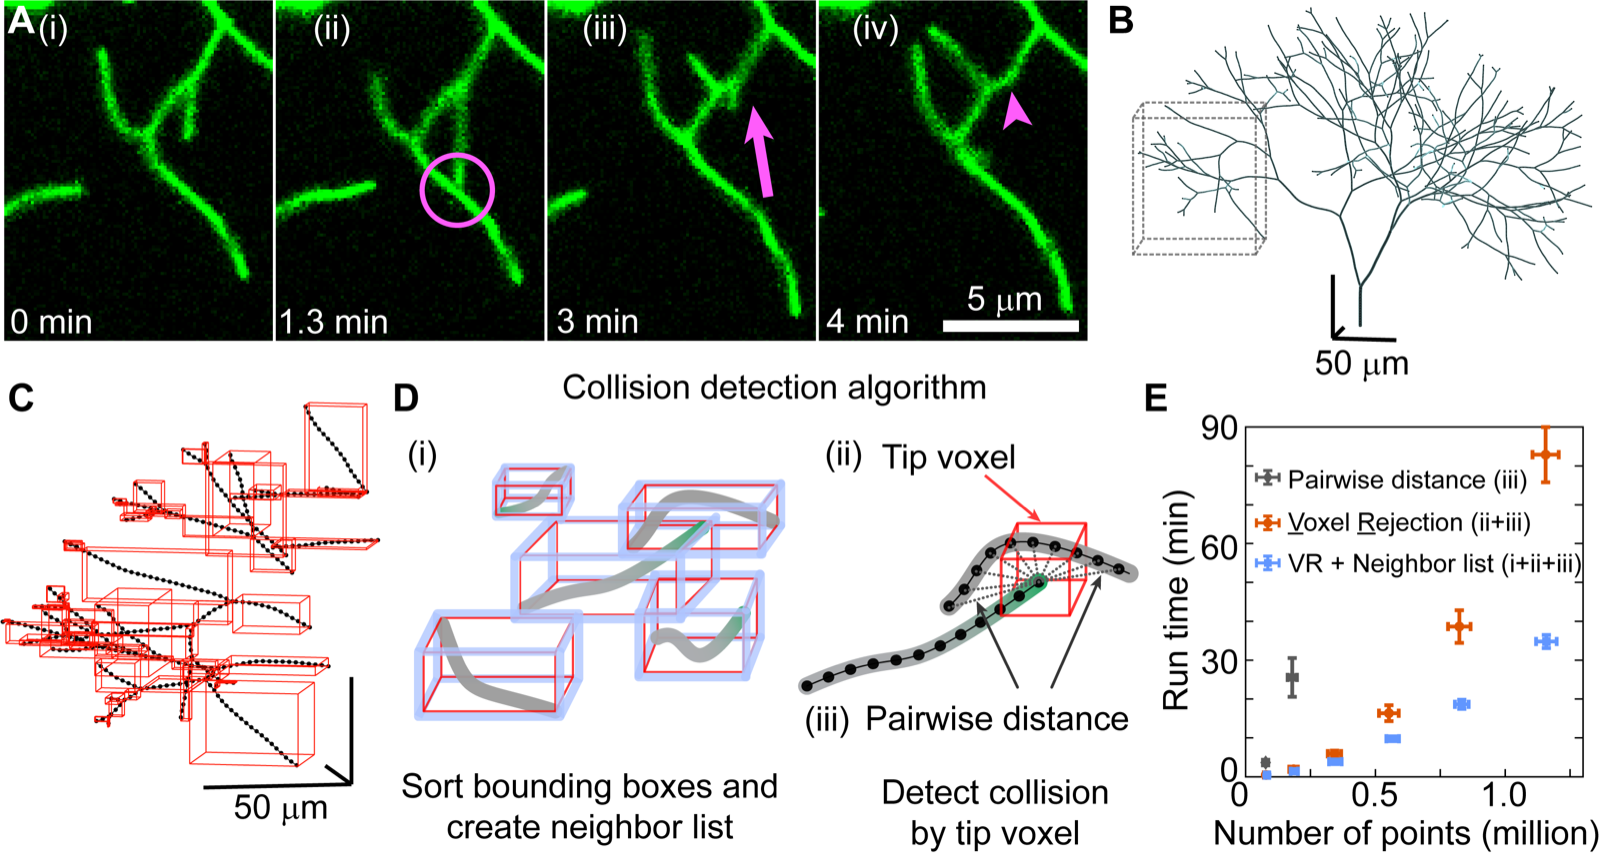
\includegraphics[width=\textwidth]{fig4_collision.png}
  \caption{\textbf{Contact interaction and the collision-detection algorithm.}
  \textbf{(A)} In vivo: a growing class~IV tip touches a neighbouring branch (circle, 1.3\,min), retracts (arrow, 3\,min) and leaves the territory (arrowhead, 4\,min).
  \textbf{(B)} A simulated arbor. The dashed box marks the region shown in C.
  \textbf{(C)} Each branch carries an axis-aligned bounding box (red).
  \textbf{(D)} The three-stage search. (i)~Bounding boxes, padded by the interaction range (blue), are sorted along one axis to build a neighbour list. (ii)~Only neighbours whose box overlaps the tip voxel are kept. (iii)~Exact point-to-tip distances are computed for the few survivors.
  \textbf{(E)} Run time against the total number of points for pairwise distance only (iii), voxel rejection (ii+iii), and voxel rejection plus neighbour list (i+ii+iii). The full scheme is roughly an order of magnitude faster at $10^6$ points.}
  \label{fig:collision}
\end{figure}

\paragraph{Physics.}
Class~IV dendrites tile the body wall and avoid their own branches. A growing tip that touches another branch of the same cell usually stalls or retracts. This self-avoidance is mediated by Dscam and related recognition molecules~\cite{Matthews2007}. Contact-based retraction alone is enough to set the mesh size of the arbor~\cite{Ganguly2016}.

We model a contact as follows. A tip at $\vect x_\text{tip}$ on branch $i$ collides with branch $j$ when some point $\vect y\in j$ satisfies
\begin{equation}
  \lVert\vect x_\text{tip}-\vect y\rVert\le r_i+r_j+d_\text{th},
\end{equation}
where $d_\text{th}$ is \code{Interaction\_Threshold}.

After a contact:
\begin{itemize}
  \item The branch switches immediately to the most retracting state of the collision state set, i.e.\ the state with minimum velocity.
  \item For a period $T_c$ (\code{PostCollisionPeriod}) it evolves with its own Markov chain (\code{Collision\_TransitionRates}). This one mechanism covers both observed fates:
  \begin{itemize}
    \item \textbf{stall}: the collision dynamics stay mostly in the pause state;
    \item \textbf{retraction}: the collision dynamics stay mostly in the shrink state, often all the way back to the branch point, after which the branch is deleted.
  \end{itemize}
  \item After $T_c$ the branch returns to free dynamics in state~1.
  \item With \code{FreezeCollidedBranch=true}, a branch in contact also cannot spawn new branches.
\end{itemize}

\paragraph{Why a special algorithm is needed.}
A tree with $N$ points and $M$ dynamic tips needs $O(MN)\sim O(N^2)$ distance evaluations per step if checked naively. With $N\sim10^6$ and $10^5$ steps this is far too slow (Fig.~\ref{fig:collision}E). BranchMorphoGen therefore uses a classic broad-phase/narrow-phase scheme adapted to tree geometry.

\paragraph{Stage (i): sort-and-sweep neighbour lists.}
\code{Simulation::updateNeighborList} (Algorithm~\ref{alg:neigh}) works as follows:
\begin{enumerate}
  \item Find the axis of greatest spatial extent of the whole tree.
  \item Sort all branch AABBs by their lower coordinate along that axis.
  \item For each dynamic branch, inflate its box by the padding $\delta=d_\text{th}+r_\text{min}$ and sweep forward through the sorted list. Skip boxes that end before the window, and stop as soon as a box starts beyond it.
  \item Keep every box that overlaps the window in all three axes.
\end{enumerate}
Sorting costs $O(B\log B)$ for $B$ branches, and each sweep visits only the boxes inside its window.

Because tips move at most $v_\text{max}\Delta t$ per step, the list stays valid for about $\delta/(v_\text{max}\Delta t)$ steps, like the ``skin'' of a Verlet list in molecular dynamics. The rebuild interval $n_\text{coll}$ is set from this estimate, rounded to a multiple of 5 and kept between 5 and 10 steps. Each branch's parent and sibling are always included in its list.

\begin{algorithm}[!htbp]
\caption{Broad phase: sort-and-sweep neighbour lists (\code{updateNeighborList})}\label{alg:neigh}
\begin{algorithmic}[1]
\State $a\gets\arg\max_{\alpha\in\{x,y,z\}}$ (extent of the union of all AABBs along $\alpha$)
\State $\sigma\gets$ branch indices sorted by $\text{AABB}_\text{min}[a]$
\ForAll{dynamic branches $i$}
  \State $\mathcal N_i\gets\{i,\text{parent}(i),\text{sibling}(i)\}$; $W\gets\text{AABB}_i$ inflated by $\delta$
  \For{$j$ in order $\sigma$}
     \If{$\text{AABB}_j.\max[a]<W.\min[a]$} \textbf{continue} \EndIf
     \If{$\text{AABB}_j.\min[a]>W.\max[a]$} \textbf{break} \EndIf \Comment{early exit}
     \If{$W\cap\text{AABB}_j\neq\emptyset$} $\mathcal N_i\gets\mathcal N_i\cup\{j\}$ \EndIf
  \EndFor
\EndFor
\end{algorithmic}
\end{algorithm}

\paragraph{Stages (ii) and (iii): tip voxel and exact distance.}
At each growth attempt, \code{BranchCollision::\allowbreak checkBranchCollision} loops only over $\mathcal N_i$:
\begin{itemize}
  \item A cube of half-width $r_i+r_j+d_\text{th}$ around the tip (the ``tip voxel'') is tested against $\text{AABB}_j$, which rejects most candidates in $O(1)$.
  \item For the survivors, squared distances to the points of $j$ are computed. The loop exits at the first hit.
  \item Branches next to the tip in the tree need special care, or a tip would always ``collide'' with its own base. For the branch itself, its parent and its sibling, two rules apply:
  \begin{itemize}
    \item contact needs the smaller distance $d_\text{th}$;
    \item the $n_\text{oth}=\lceil(r_i+r_j+d_\text{th})/\Delta s\rceil$ points nearest the shared junction are skipped.
  \end{itemize}
\end{itemize}
Together, the three stages bring the cost per step close to $O(M\bar k)$, where $\bar k$ is the average number of neighbours, plus an $O(B\log B)$ sort every few steps.

\paragraph{Soma and boundary contacts.}\label{sec:boundary}
\begin{itemize}
  \item \textbf{Soma.} A tip that enters the soma ($\lVert\vect x-\vect x_\text{root}\rVert\le R_s$) collides.
  \item \textbf{Boundary.} Outside the hard box a tip collides at random, so the walls are soft. Along each axis $\alpha$, the collision rate rises smoothly with the distance outside the box:
  \begin{equation}
    p_\alpha(\vect x)=\tfrac12\left[1+\operatorname{erf}\!\left(\frac{|x_\alpha-c_\alpha|-w_\alpha}{\ell_s}\right)\right],\qquad
    w_\alpha=\tfrac12(x_{\alpha,+}-x_{\alpha,-})+2\ell_s .
  \end{equation}
  Here $c_\alpha$ is the centre of the box and $\ell_s$ is \code{Boundary\_SoftLength}. The tip collides in a step with probability $\max_\alpha p_\alpha\,\Delta t$. The soft wall avoids the artificial pile-up of tips along a hard wall, and mimics the gradual confinement by the neighbouring cells and the segment border.
\end{itemize}

\FloatBarrier
%---------------------------------------------------------------------
\subsection{Branch deletion and topology repair}\label{sec:topology}
%---------------------------------------------------------------------
When a terminal branch retracts completely it is queued for deletion. After all growth and branching in a step, \code{BranchRelabel::debranching} processes the queue:
\begin{enumerate}
  \item \textbf{Merge.} Removing a child leaves its parent with a single child, so the junction is no longer a branch point. The sibling's points are joined onto the end of the parent. The parent inherits the sibling's state, velocity, collision clock and children (\code{mergeTipsAfterDeletion}). This keeps the tree strictly binary and avoids zero-length segments.
  \item \textbf{Both children deleted.} If the sibling is being deleted too, the parent becomes a dynamic tip again, in the growing state.
  \item \textbf{Relabel.} Surviving branches are compacted into a new array. Every parent, sibling, child and neighbour index is remapped in a single $O(B)$ pass with a lookup table from old to new indices (\code{relabelIndex}).
\end{enumerate}

\FloatBarrier
%---------------------------------------------------------------------
\subsection{Diameter scaling}\label{sec:radius}
%---------------------------------------------------------------------
\paragraph{Physics.}
Branch diameters decrease from the soma to the tips according to scaling laws whose exponent reflects the function of the network. Examples:
\begin{itemize}
  \item Rall's 3/2 law, $r_p^{3/2}=\sum r_d^{3/2}$~\cite{Rall1959};
  \item Murray's cube law~\cite{Murray1926};
  \item the area-preserving rule of da Vinci, $r_p^2=\sum r_d^2$.
\end{itemize}
BranchMorphoGen supports a family of ``supply'' models. The cross-sectional area of branch $i$ grows linearly with an additive quantity $Q_i$ of the subtree it supports:
\begin{equation}
  \pi r_i^2 = \pi r_\text{min}^2+\beta\,Q_i \quad\Longrightarrow\quad
  r_i=\min\!\left(\sqrt{r_\text{min}^2+\beta Q_i/\pi},\;r_\text{max}\right),
  \label{eq:radius}
\end{equation}
where $\beta$ is \code{BetaRadius}. Available choices of $Q_i$ (\code{RadiusModel}):
\begin{itemize}
  \item the number of tips (\code{TipNumber});
  \item the number of branches (\code{BranchNumber});
  \item total length $\sum L$ (\code{Length});
  \item surface area $\sum\pi r L$ (\code{Area});
  \item volume $\sum\pi r^2L$ (\code{Volume});
  \item none, i.e.\ a constant radius (\code{None}).
\end{itemize}
Because $Q$ is additive over subtrees, $Q_p=Q_{d_1}+Q_{d_2}$ at a junction for the tip-number model. Eq.~\eqref{eq:radius} then gives $r_p^2-r_\text{min}^2=(r_{d_1}^2-r_\text{min}^2)+(r_{d_2}^2-r_\text{min}^2)$, which is da Vinci's area-preserving rule with an offset $r_\text{min}$. This ``pipe model'' fits the narrowing of class~IV dendrites well, where the area of a branch is proportional to the number of tips it supports.

\paragraph{Algorithm.}
All $Q_i$ are computed in one depth-first, post-order traversal that visits each branch and each edge exactly once (Algorithm~\ref{alg:radius}, \code{BranchTopology::updateRadius}). The total cost is $O(B)$. The radii are refreshed every $n_F=\max(5,\lfloor1/\Delta t\rfloor)$ steps, together with the mechanics.

\begin{algorithm}[!htbp]
\caption{Subtree statistics and radius update (\code{BranchTopology})}\label{alg:radius}
\begin{algorithmic}[1]
\Function{Visit}{$i$}
  \If{visited$[i]$} \textbf{return} \EndIf; visited$[i]\gets$ true
  \State $n_\text{br}[i]\gets1$; $\Lambda[i]\gets L_i$; $A[i]\gets\pi r_iL_i$; $V[i]\gets\pi r_i^2L_i$
  \If{$i$ is internal with children $c_1,c_2$}
     \State \Call{Visit}{$c_1$}; \Call{Visit}{$c_2$}
     \State add the children's $n_\text{br},\Lambda,A,V$ to $i$; $n_\text{tip}[i]\gets n_\text{tip}[c_1]+n_\text{tip}[c_2]$
  \Else\ $n_\text{tip}[i]\gets1$
  \EndIf
\EndFunction
\State \textbf{for all} $i$: \Call{Visit}{$i$}; \textbf{then for all} $i$: set $r_i$ by Eq.~\eqref{eq:radius}
\end{algorithmic}
\end{algorithm}

\FloatBarrier
%---------------------------------------------------------------------
\subsection{Branch mechanics and straightening}\label{sec:mech}
%---------------------------------------------------------------------
\begin{figure}[!htbp]
  \centering
  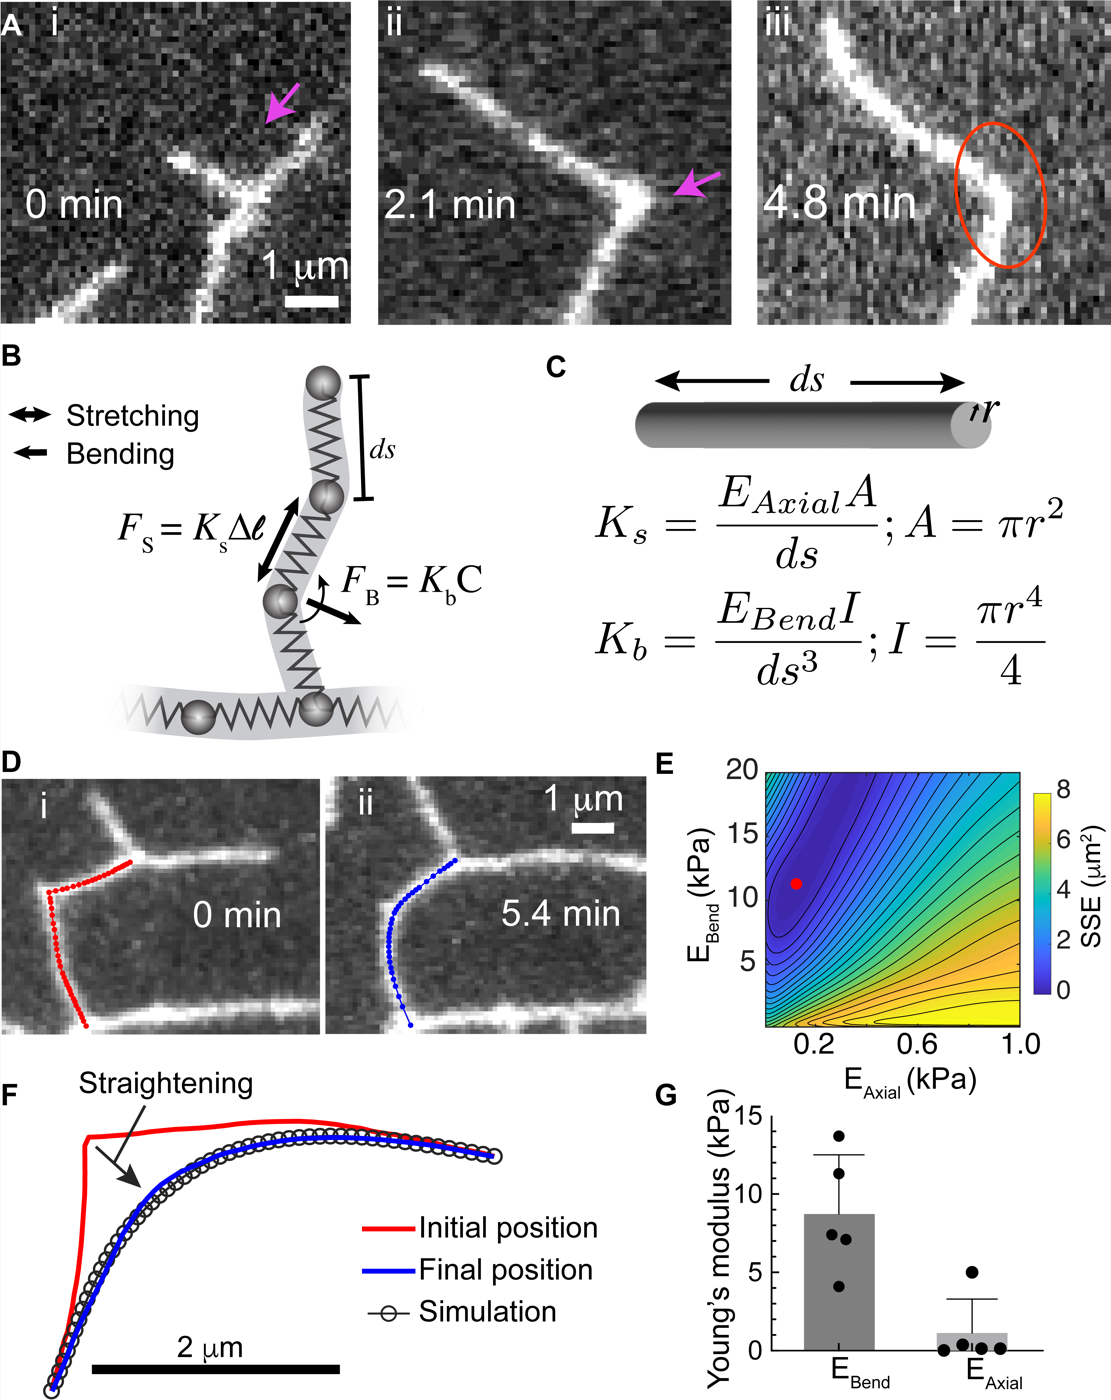
\includegraphics[width=0.80\textwidth]{fig5_straightening.png}
  \caption{\textbf{Branch straightening and the mechanical model.}
  \textbf{(A)} In vivo: after a lateral branch forms (arrows), the sharp corner at the branch point relaxes into a smooth curve (red ellipse) within minutes.
  \textbf{(B)} Bead--spring representation. Neighbouring points are joined by stretching springs, $F_S=K_s\Delta\ell$, and every triplet resists bending, $F_B=K_bC$.
  \textbf{(C)} The stiffnesses come from a cylinder of radius $r$ and segment length $ds$: $K_s=E_\text{Axial}A/ds$ with $A=\pi r^2$, and $K_b=E_\text{Bend}I/ds^3$ with $I=\pi r^4/4$.
  \textbf{(D)} A tracked branch at 0\,min (red) and after straightening at 5.4\,min (blue).
  \textbf{(E)} Sum of squared errors (SSE) between the simulated and observed final shape as a function of $(E_\text{Axial},E_\text{Bend})$. The red dot is the best fit.
  \textbf{(F)} Initial shape (red), final shape (blue) and simulation (circles) for the best fit.
  \textbf{(G)} Fitted moduli over $n=5$ events: $E_\text{Bend}\approx9$\,kPa and $E_\text{Axial}\approx1$\,kPa.}
  \label{fig:mech}
\end{figure}

\paragraph{Physics.}
Branching and retraction alone leave sharp kinks and zig-zags, which real dendrites do not show. Time-lapse imaging shows that corners relax within minutes (Fig.~\ref{fig:mech}A). We therefore treat each branch as a slender elastic rod in a viscous environment.

With $\Delta s=$\,\code{BranchInterval} as the rest length, the discrete elastic energy is
\begin{equation}
  U=\sum_{\text{segments }(j,j+1)}\frac{k_s}{2}\big(\lVert\vect x_{j+1}-\vect x_j\rVert-\Delta s\big)^2
   +\sum_{\text{triplets }(j-1,j,j+1)}\frac{k_b}{2}\,\big\lVert\vect x_{j-1}-2\vect x_j+\vect x_{j+1}\big\rVert^2 ,
  \label{eq:energy}
\end{equation}
\begin{equation}
  k_s=\frac{E_\text{ax}\,\pi r^2}{\Delta s},\qquad k_b=\frac{E_\text{bend}\,\pi r^4/4}{\Delta s^3}.
\end{equation}
The second sum is the discrete form of the Euler--Bernoulli bending energy $\tfrac{EI}{2}\int\kappa^2\,\dd s$, using the curvature estimate $\kappa\simeq\lVert\vect x_{j-1}-2\vect x_j+\vect x_{j+1}\rVert/\Delta s^2$.

Bending triplets also span the junctions: (parent tip, child base, child point) and (child, branch point, child). Branch points therefore transmit torque, and a freshly formed corner relaxes. The base of each primary branch is tied to the root by a stiff ``ground spring'' of stiffness $k_s$.

At cellular scales inertia is negligible, so the dynamics are overdamped:
\begin{equation}
  \zeta\,\dot{\vect x}_j=-\frac{\partial U}{\partial\vect x_j},\qquad \zeta=4\pi\,\Delta s\,\eta,
\end{equation}
where $\zeta$ is the Stokes-like drag on a segment and $\eta$ is \code{DragCoef}.

The bending relaxation time of a mode of wavelength $\lambda$ scales as $\tau\sim\zeta\lambda^4/(\Delta s\,E_\text{bend}I)\propto r^{-4}$. Thick branches therefore straighten much faster than thin ones. Combined with diameter scaling (Sec.~\ref{sec:radius}), this coupling turns thick branches, which support many tips, into long straight ``primary'' branches, while thin terminal branches stay tortuous. A hierarchy of primary, secondary and higher-order branches thus emerges without being imposed.

\paragraph{Parameter estimation.}
$E_\text{ax}$ and $E_\text{bend}$ were fitted by simulating real straightening events. We started from the traced initial shape and minimised the sum of squared distances to the traced final shape over a grid of moduli (Fig.~\ref{fig:mech}E--G). Note that the values in \code{parameters.in} are in the simulation's own units (lengths in \textmu m, times in min, unit drag); they are not in kPa.

\paragraph{Algorithm: semi-implicit global solve.}
Bending is numerically \emph{stiff}. Since $k_b\propto\Delta s^{-3}$, an explicit Euler step would need $\Delta t\lesssim\zeta/(16k_b)$, which is far smaller than the growth time step. \code{BranchForces::\allowbreak updatePosition\_\allowbreak ImplicitGlobal} therefore uses an implicit--explicit (IMEX) scheme over the whole tree at once:
\begin{itemize}
  \item \textbf{Implicit bending.} The bending term is quadratic, so its Hessian is a constant matrix, $\mathbf K_b=\sum k_b\,\mathbf L^\top\mathbf L$, built from the stencil $\mathbf L=[1,-2,1]$. It is assembled as a sparse $3N\times3N$ matrix and treated implicitly.
  \item \textbf{Explicit stretching.} The nonlinear stretching force is treated explicitly. To keep that step stable, the spring extension is softly saturated: $F=k_s\,\ell_\text{m}\tanh\!\big((d-\Delta s)/\ell_\text{m}\big)$ with $\ell_\text{m}=0.9\,\Delta s$.
  \item \textbf{Linear solve.} With $\mu=1/\zeta$ and $\Delta t'=n_F\Delta t$ (mechanics runs every $n_F$ steps), each update solves
  \begin{equation}
    \big(\mathbf I+\mu\Delta t'\,\mathbf K_b+\mu\Delta t'\,\mathbf K_\text{root}\big)\,\vect X^{n+1}
    =\vect X^{n}+\mu\Delta t'\,\vect F_s(\vect X^{n})+\mu\Delta t'\,\mathbf K_\text{root}\vect X_\text{root}.
  \end{equation}
  The matrix is symmetric positive definite, so it is factorised by sparse Cholesky ($\mathbf{LDL}^\top$, Eigen \code{SimplicialLDLT}). Because the bending term is treated implicitly, this step is unconditionally stable for any $\Delta t'$.
\end{itemize}

\begin{algorithm}[!htbp]
\caption{Semi-implicit mechanics update (\code{updatePosition\_ImplicitGlobal})}\label{alg:mech}
\begin{algorithmic}[1]
\State assign a global index to every point; pack the positions into $\vect X^n\in\mathbb R^{3N}$
\State triplets $\gets$ identity; add ground springs $\mu\Delta t'k_s$ at the base of each primary branch
\ForAll{branches $b$}
   \State add $\mu\Delta t' k_b(r_b)\,\mathbf L^\top\mathbf L$ blocks for interior triplets and the junction triplets (parent--child, child--child)
\EndFor
\State $\mathbf A\gets$ sparse matrix from triplets; factorise $\mathbf A=\mathbf{LDL}^\top$
\State $\vect F_s\gets$ saturated stretching forces from $\vect X^n$ (including across junctions)
\State solve $\mathbf A\vect X^{n+1}=\vect X^n+\mu\Delta t'\vect F_s+\text{(root terms)}$
\State scatter $\vect X^{n+1}$ back into the branches; move children's base points; update lengths and AABBs
\end{algorithmic}
\end{algorithm}

\FloatBarrier
%---------------------------------------------------------------------
\subsection{Synthetic microscopy images}\label{sec:tiff}
%---------------------------------------------------------------------
To provide ground-truth data for segmentation and tracing algorithms, every output frame is also rendered as a 16-bit TIFF in the plane \code{ImagePlane} (\code{src/PrintTIFF.cpp}). The steps are:
\begin{enumerate}
  \item \textbf{Rasterise.} Each segment is sampled at sub-pixel spacing. Every sample paints a disc of radius $r_i$, with pixel size \code{pixelsize}. Each painted pixel adds an intensity drawn from $\mathcal N\big(\text{Poisson}(r_i\bar S),\,r_i\sigma_S\big)$, where $\bar S$ is \code{SignalMean} and $\sigma_S$ is \code{SignalStd}. This mimics photon shot noise, and thicker branches come out brighter. Samples inside the parent's radius are skipped so that junctions are not counted twice.
  \item \textbf{Blur.} The image is convolved with a Gaussian point-spread function of width $\sigma_\text{PSF}=1.5$ pixels.
  \item \textbf{Background.} A noisy background $\mathcal N(\bar B,\sigma_B)$ is added, from \code{BackgroundMean} and \code{BackgroundStd}, on a fixed offset of 100 counts.
\end{enumerate}
The field of view is either \code{MAX\_IMAGE\_SIZE} centred on the root, or the final simulation box plus the soft margin (\code{MAX\_IMAGE\_SIZE}$=-1$).

\FloatBarrier
%---------------------------------------------------------------------
\subsection{Time-dependent parameters}\label{sec:timedep}
%---------------------------------------------------------------------
Development is not stationary: tip speeds, switching rates and branching rates change as the larva grows. Any of \code{LimitsX/Y/Z}, \code{StateVelocity}, \code{TransitionRates} and \code{BranchingRate} may therefore be given as a table of \code{time:value} pairs. The values are interpolated linearly (\code{InterpolatedParameter.h}) and evaluated once per step. \code{inf} and \code{-inf} are accepted as times.

Table~\ref{tab:classiv} lists the class~IV values shipped in \code{parameters.in}.

\begin{table}[!htbp]
\centering\small
\caption{Measured, time-dependent tip dynamics and branching rates used for \emph{Drosophila} class~IV neurons (\code{parameters.in}). The states are growth (G), pause (P) and shrinkage (S). Time is in minutes after egg laying (960\,min = 16\,h, 7200\,min = 120\,h). Velocities are in \textmu m/min; rates are in min$^{-1}$, and the branching rate is per \textmu m.}
\label{tab:classiv}
\begin{tabular}{@{}rccccccccc@{}}
\toprule
$t$ & $v_G$ & $v_S$ & $K_{GP}$ & $K_{GS}$ & $K_{PG}$ & $K_{PS}$ & $K_{SG}$ & $K_{SP}$ & $k_b$\\
\midrule
960  & 1.54 & $-1.63$ & 0.696 & 0.509 & 0.423 & 0.296 & 0.669 & 0.710 & 0.0191\\
1440 & 1.60 & $-1.53$ & 0.784 & 0.640 & 0.335 & 0.314 & 0.598 & 0.946 & 0.0095\\
2880 & 1.60 & $-1.10$ & 0.933 & 0.435 & 0.155 & 0.235 & 0.282 & 1.251 & 0.0019\\
5760 & 1.64 & $-1.33$ & 0.923 & 0.799 & 0.116 & 0.117 & 0.575 & 1.276 & 0.0011\\
\bottomrule
\end{tabular}
\end{table}

\FloatBarrier
%---------------------------------------------------------------------
\subsection{Randomness, reproducibility and parallelism}
%---------------------------------------------------------------------
All random numbers come from one generator per sample (\code{RandomUtils}), seeded with $\texttt{GLOBAL\_SEED}+i$ for sample $i$, where \code{GLOBAL\_SEED}$=65$ in \code{src/main.cpp}. Identical input files therefore give bit-identical trees. To get a new ensemble, change the seed or raise \code{NSample}.

With \code{RunParallel=true} and \code{NSample}$>1$, the samples run in separate \code{std::thread}s. Each thread has its own copy of the parameters and its own generator. The only shared resource is the run-time log, which is protected by a mutex.

%=====================================================================
\section{Results: what the framework can generate}
%=====================================================================
\begin{figure}[!htbp]
  \centering
  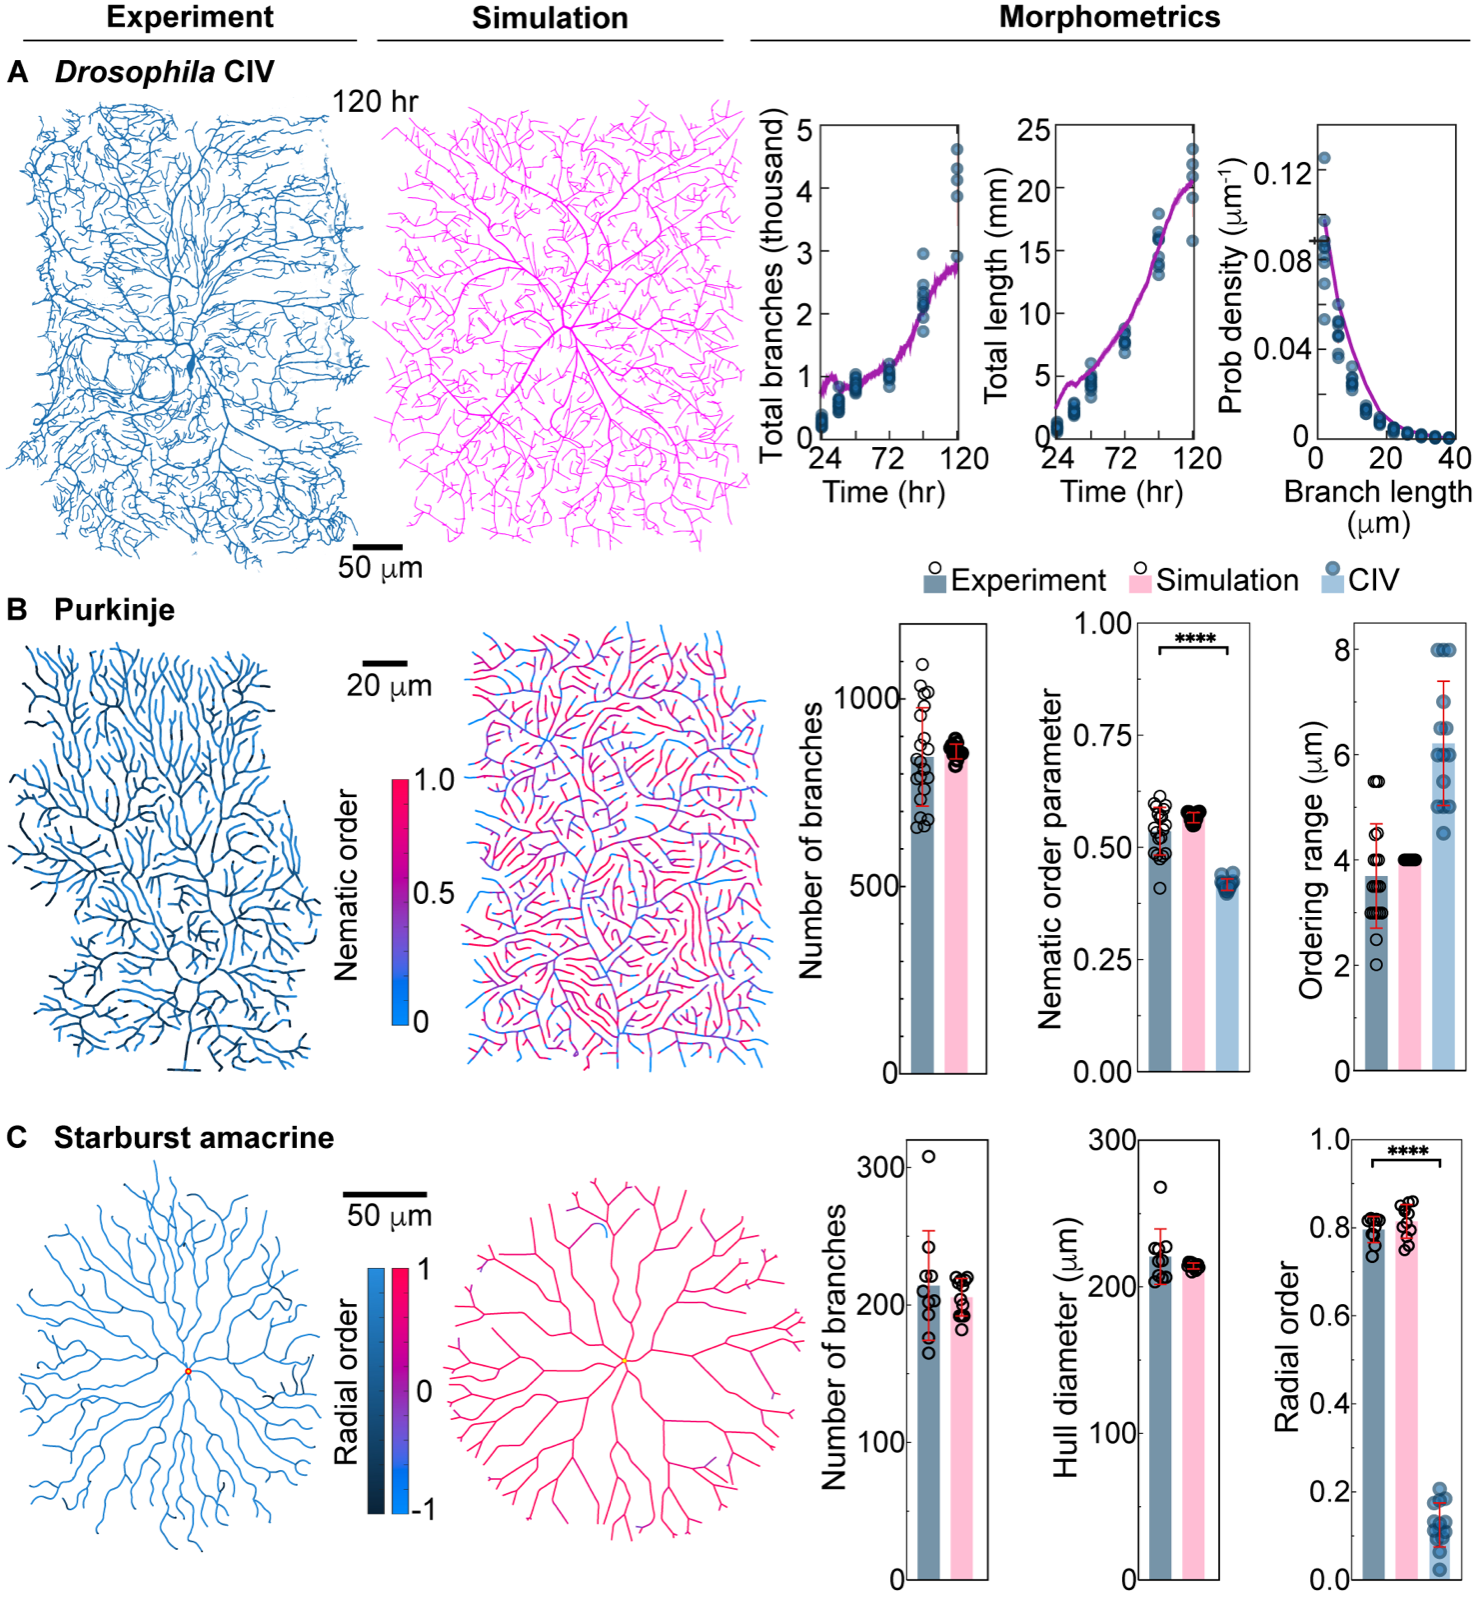
\includegraphics[width=0.97\textwidth]{fig6_neurons.png}
  \caption{\textbf{BranchMorphoGen reproduces several neuronal morphologies quantitatively.} Columns: experiment, simulation, morphometrics.
  \textbf{(A)}~\emph{Drosophila} class~IV da neuron at 120\,h. The simulated total branch number, total length and branch-length distribution (purple) follow the measurements (dots) throughout larval development (24--120\,h).
  \textbf{(B)}~Purkinje cell. The local nematic order of branch orientations is colour-coded. The simulation matches the experimental branch number, nematic order parameter and ordering range. These are clearly different from class~IV (light blue), which is much less ordered.
  \textbf{(C)}~Starburst amacrine cell. Branches are colour-coded by radial order, the alignment with the radial direction. The simulation matches the branch number and hull diameter, and reproduces the high radial order ($\approx0.8$), unlike class~IV neurons ($\approx0.1$).}
  \label{fig:neurons}
\end{figure}

\paragraph{Drosophila class~IV neurons (Fig.~\ref{fig:neurons}A).}
These neurons are produced by the following combination:
\begin{itemize}
  \item three-state tip dynamics with the time-dependent rates of Table~\ref{tab:classiv};
  \item length-dependent lateral branching at about $90^\circ$ in the local frame;
  \item contact-induced retraction;
  \item tip-number diameter scaling and straightening;
  \item a box that expands from $80\times120$\,\textmu m at 16\,h to $350\times450$\,\textmu m at 96\,h.
\end{itemize}
The simulation reproduces the measured growth of the number of branches and the total length over five days, and the exponential-like branch-length distribution.~\cite{Shree2022,Ouyang2025}.

\paragraph{Purkinje cells (Fig.~\ref{fig:neurons}B).}
Purkinje dendrites are planar and locally aligned. This \emph{nematic} order comes from global-frame branching with a narrow, reflective azimuthal angle, together with strong self-avoidance in a thin box ($|z|$ small). The nematic order parameter measures how well neighbouring branch orientations align (in 2-D, e.g.\ $S=\langle\cos2(\phi-\phi_0)\rangle$ with $\phi_0$ the local director). The ordering range is the length scale over which this order decays.

\paragraph{Starburst amacrine cells (Fig.~\ref{fig:neurons}C).}
Radially symmetric, planar arbors with high radial order, $\langle\hat{\vect t}\cdot\hat{\vect r}\rangle\approx0.8$, come from tip bifurcation in the local frame with a long persistence length. Branches then keep their outward direction from the central soma.

\begin{figure}[!htbp]
  \centering
  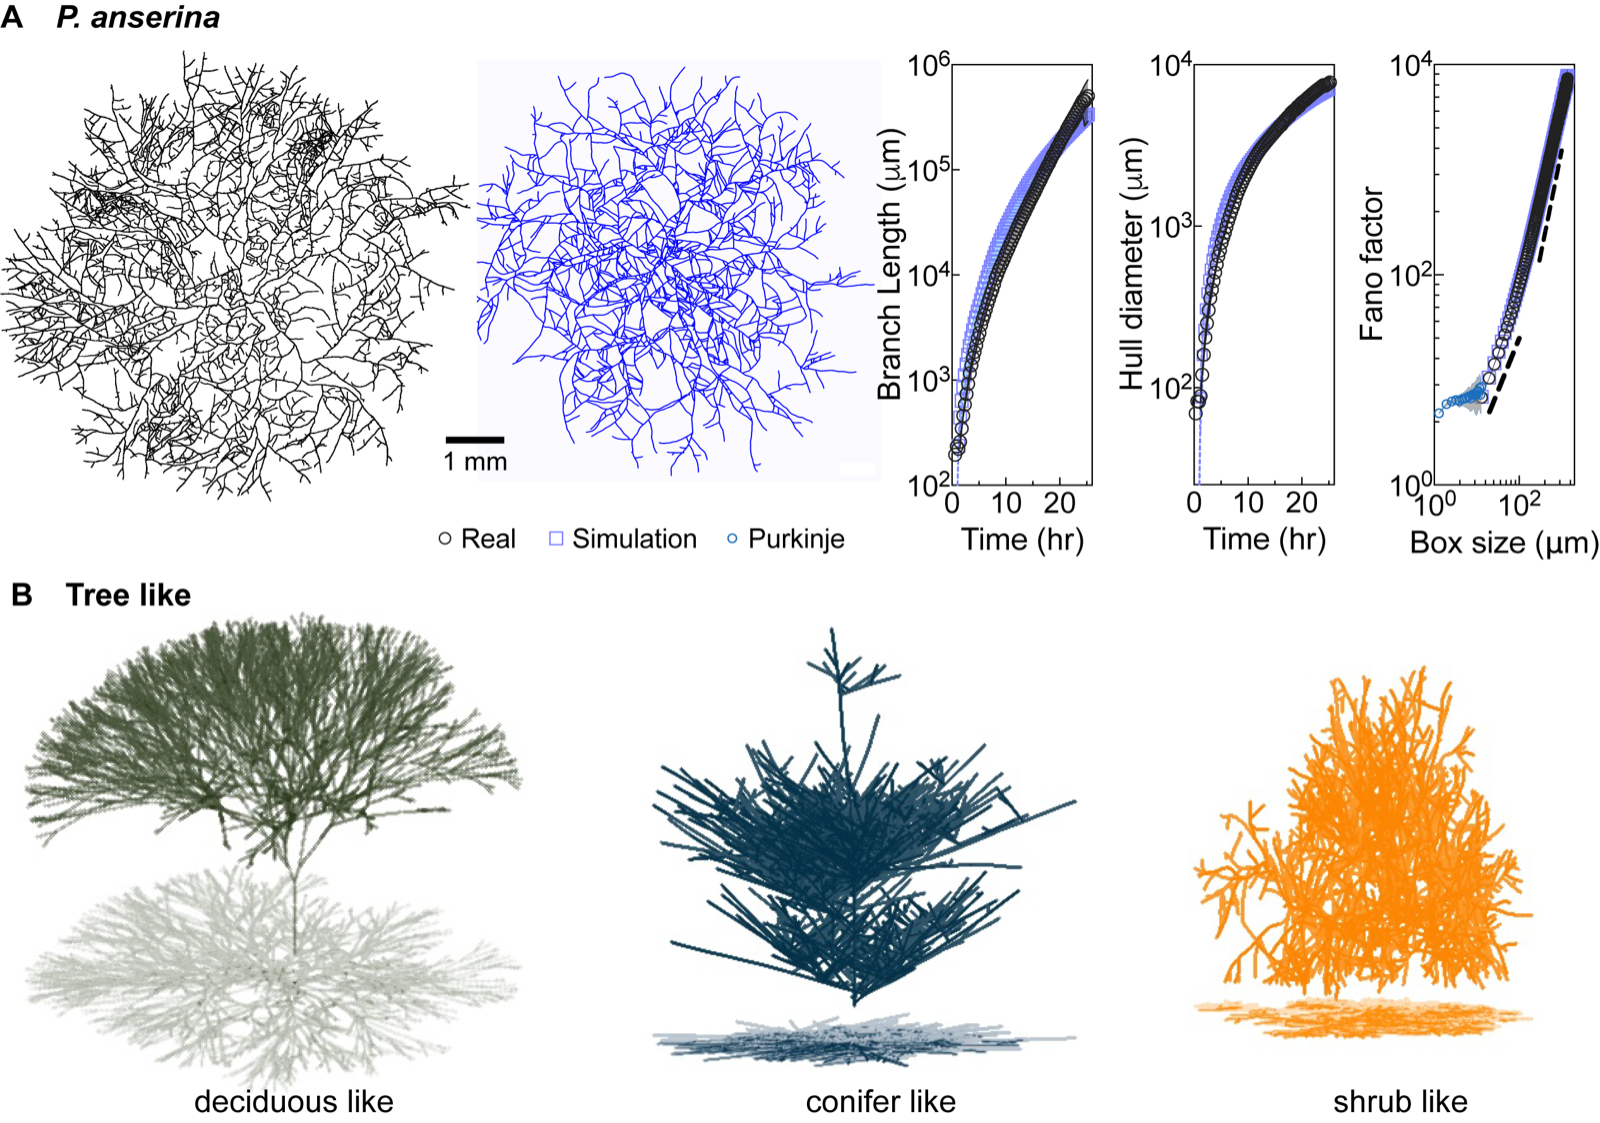
\includegraphics[width=0.97\textwidth]{fig7_non_neurons.png}
  \caption{\textbf{Non-neuronal branched networks across length and time scales.}
  \textbf{(A)}~Mycelium of the filamentous fungus \emph{Podospora anserina}~\cite{Dikec2020,Ledoux2022}: experiment (black) and simulation (blue). Total branch length and hull diameter over 25\,h overlap the data across four decades. The Fano factor against box size matches the real colony at large scales, and differs from Purkinje cells (small blue circles).
  \textbf{(B)}~Three-dimensional ``tree-like'' architectures (shadows show projections) obtained by changing only the polar/azimuthal angles, the persistence length and the branching mode: deciduous-like, conifer-like and shrub-like.}
  \label{fig:nonneurons}
\end{figure}

\paragraph{Fungi and plants (Fig.~\ref{fig:nonneurons}).}
Because the modules are generic, the same code covers networks millimetres across and hours long:
\begin{itemize}
  \item \textbf{Fungal mycelium.} Fungal hyphae grow with nearly constant tip speed (a one-state model), branch laterally and do not retract on contact. A model with \code{SelfAvoiding=false}, a long persistence length and millimetre-scale limits reproduces the growth of \emph{P.~anserina} colonies.
  \item \textbf{3-D plant shapes.} In three dimensions, changing the polar angle (apical dominance), the branching mode and $L_p$ moves between deciduous-, conifer- and shrub-like crowns, as in classic geometric models of trees~\cite{Honda1971}.
\end{itemize}

%=====================================================================
\section{Using BranchMorphoGen}\label{sec:usage}
%=====================================================================
\subsection{Installation}
\paragraph{Requirements.}
\begin{itemize}
  \item CMake $\ge$3.16;
  \item a C++17 compiler (GCC or Clang);
  \item libtiff with development headers;
  \item POSIX threads.
\end{itemize}
Eigen is bundled in \code{third\_party/eigen}. The optional web GUI needs only Python $\ge$3.8.

\begin{lstlisting}[language=bash]
# dependencies
sudo apt-get install libtiff-dev        # Ubuntu/Debian
brew install libtiff                    # macOS
export TIFF_ROOT=/path/to/tiff          # only for non-standard locations

# build
git clone https://github.com/SabyasachiSutradhar/BranchMorphoGen.git
cd BranchMorphoGen && mkdir build && cd build
cmake ..            # or: cmake -DTIFF_ROOT=/custom/tiff ..
make -j
./BranchMorphoGen --about               # prints version and build date
\end{lstlisting}

\subsection{Running}
\begin{lstlisting}[language=bash]
mkdir -p runs/test1 && cd runs/test1
/path/to/build/BranchMorphoGen /path/to/parameters.in
\end{lstlisting}
All output is written to the \emph{current working directory}, prefixed by \code{SimulationName}. Use one folder per run.

Runs are non-interactive, so parameter scans are easy to script:
\begin{lstlisting}[language=bash]
for kb in 0.005 0.01 0.02; do
  d=runs/kb_$kb; mkdir -p $d
  sed "s/^\(\s*BranchingRate\s*=\).*/\1 $kb;/" parameters.in > $d/p.in
  (cd $d && ../../build/BranchMorphoGen p.in) &
done; wait
\end{lstlisting}

\subsection{Input-file syntax}
\begin{itemize}
  \item One \code{Key = value;} per line. Comments start with \code{//}, \code{\#} or \code{\%}.
  \item Keys are case-sensitive. An unknown key prints \code{Warning: Unknown key} and is ignored.
  \item Vectors are comma-separated, e.g.\ \code{States = 1,0,-1;}.
  \item Matrices use \code{;} between rows and \code{,} within a row, e.g.\ \code{0,0.7,0.5; 0.4,0,0.3; 0.7,0.7,0}.
  \item Booleans: \code{true}/\code{false}.
  \item \code{inf} is accepted for \code{PersistanceLength} and \code{PostCollisionPeriod}.
  \item Time-dependent parameters take one \code{t:value;} per line, and must not mix constants and tables:
\end{itemize}
\begin{lstlisting}
BranchingRate =
960:0.01906;
1440:0.00954;
7200:0.00114;
LimitsZ = -10,10;          // constant
\end{lstlisting}

\subsection{Parameter reference}
Defaults are the class~IV values in \code{parameters.in}. Lengths are in \code{SpatialUnit} (\textmu m) and times in \code{TemporalUnit} (min). ``TD'' marks parameters that can depend on time.

{\small
\setlength{\LTcapwidth}{\textwidth}
\begin{longtable}{@{}p{4.1cm}p{2.6cm}p{8.6cm}@{}}
\toprule
\textbf{Key} & \textbf{Example} & \textbf{Meaning}\\ \midrule\endhead
\bottomrule\endfoot
\multicolumn{3}{@{}l}{\emph{Simulation and time}}\\
\code{SimulationName} & \code{xx} & Prefix of all output files\\
\code{SpatialUnit}, \code{TemporalUnit} & \code{micron}, \code{min} & Labels written to the outputs\\
\code{NSample} & 1 & Independent samples (seed $65+i$)\\
\code{RunParallel} & \code{false} & One thread per sample\\
\code{Dimension} & 2 & 2 or 3\\
\code{Dt} & 0.025 & Time step $\Delta t$\\
\code{Time\_Start}, \code{Time\_End} & 960, 7200 & $T_i$, $T_f$\\
\multicolumn{3}{@{}l}{\emph{Initial configuration}}\\
\code{ReadFromSWC}, \code{SWCFileName} & \code{false}, file & Start from an SWC file or folder (one sample per file)\\
\code{Root} & 0,0,0 & Soma centre\\
\code{N\_BranchInitial} & \code{2-4} & Number of primary branches, a value or a range\\
\code{InitialLength} & 15 & Length of the primary branches\\
\code{InitialAngle}, \code{InitialAngleWithZ} & 90, 0 & Orientation of the first branch, in degrees (negative = random)\\
\code{RadiusSoma} & 5 & $R_s$\\
\code{NascentBranchLength} & 0.6 & Initial length of a new branch\\
\code{BranchInterval} & 0.1 & Point spacing $\Delta s$\\
\code{PersistanceLength} & 100 & $L_p$ (\code{inf} = straight)\\
\multicolumn{3}{@{}l}{\emph{Boundary}}\\
\code{LimitsX/Y/Z} (TD) & table & Box limits \code{min,max}\\
\code{Boundary\_SoftLength} & 15 & Soft-wall width $\ell_s$\\
\multicolumn{3}{@{}l}{\emph{Tip dynamics}}\\
\code{States} & \code{1,0,-1} & State labels\\
\code{StateVelocity} (TD) & table & $v_i$ for each state (count must match \code{States})\\
\code{TransitionRates} (TD) & $n\times n$ & $K_{ij}$, zero diagonal\\
\multicolumn{3}{@{}l}{\emph{Branching}}\\
\code{Bifurcation} & \code{false} & Tip bifurcation (\code{true}) or lateral branching (\code{false})\\
\code{BifurcationRatio} & 1.0 & Angle split $\rho$ between the daughters\\
\code{BranchingAngleRef} & \code{local} & \code{local} or \code{global} frame\\
\code{PolarAngleMode}, \code{AzimuthalAngleMode} & \code{reflective} & \code{fixed}/\code{reflective}/\code{uniform}\\
\code{PolarBranchingAngle} & 30 & Mean $\theta$ in degrees (bifurcation angle; 3-D only for lateral branching)\\
\code{AzimuthalBranchingAngle} & 90 & Mean $\varphi$ in degrees (the branching angle in 2-D)\\
\code{BranchingAngleSTD} & 30 & Angular noise $\sigma$ in degrees\\
\code{LengthDependentBranching} & \code{true} & Branching rate per unit length\\
\code{BranchingRate} (TD) & table & $k_b$\\
\code{RebranchingProb} & 0.2 & Probability that a fully retracted branch regrows instead of being deleted\\
\code{TerminationRate} & 0 & Rate at which tips become permanently static\\
\multicolumn{3}{@{}l}{\emph{Contact interaction}}\\
\code{SelfAvoiding} & \code{true} & Turn contact detection on\\
\code{Interaction\_Threshold} & 0.2 & $d_\text{th}$\\
\code{FreezeCollidedBranch} & \code{false} & Branches in contact cannot branch\\
\code{Collision\_States}, \code{Collision\_StateVelocity} & \code{1,0,-1}; \code{1.69,0,-1.1} & Post-contact states and velocities\\
\code{Collision\_TransitionRates} & $n\times n$ & Post-contact rate matrix\\
\code{PostCollisionPeriod} & 1000 & $T_c$\\
\multicolumn{3}{@{}l}{\emph{Mechanics}}\\
\code{StraightenBranches} & \code{true} & Turn the elastic relaxation on\\
\code{E\_Axial}, \code{E\_Bending} & 10, 7500 & $E_\text{ax}$, $E_\text{bend}$ (simulation units)\\
\code{DragCoef} & 0.6 & $\eta$ in $\zeta=4\pi\Delta s\,\eta$\\
\multicolumn{3}{@{}l}{\emph{Radius}}\\
\code{MinimumRadius}, \code{MaximumRadius} & 0.1, 0.4 & $r_\text{min}$, $r_\text{max}$\\
\code{RadiusModel} & \code{TipNumber} & \code{None}/\code{TipNumber}/\code{BranchNumber}/\code{Length}/\code{Area}/\code{Volume}\\
\code{BetaRadius} & 0.00135 & $\beta$ in Eq.~\eqref{eq:radius}\\
\multicolumn{3}{@{}l}{\emph{Output}}\\
\code{N\_SWC} & 11 & Number of frames written (evenly spaced)\\
\code{MAX\_IMAGE\_SIZE} & 500 & Image field of view ($-1$ = box limits)\\
\code{ImagePlane} & \code{xy} & \code{xy}/\code{xz}/\code{yz} (always \code{xy} in 2-D)\\
\code{pixelsize} & 0.1615 & Pixel size\\
\code{SignalMean}, \code{SignalStd} & 200, 20 & Branch intensity\\
\code{BackgroundMean}, \code{BackgroundStd} & 9, 2.5 & Background noise\\
\end{longtable}}

\noindent\textbf{Note.} \code{ClassIV\_parameters.in} still uses older names for the mechanics keys (\code{KSpring}, \code{KBending}, \code{Eta}), which are now ignored. It also leaves out \code{Boundary\_SoftLength} and \code{MaximumRadius}. Update it from \code{parameters.in} before use.

\subsection{Output files}
\begin{center}\small
\begin{tabularx}{\textwidth}{@{}p{5.3cm}X@{}}
\toprule
\textbf{File} & \textbf{Contents}\\ \midrule
\code{<name>-Conf-<s>-time-<t>.swc} & Morphology in standard SWC format (\code{ID Type x y z radius ParentID}). The root has ID~1 and type~1; neurite points have type~4. Readable by NEURON, neuTube, Vaa3D, the TREES toolbox and NeuroMorpho tools~\cite{Ascoli2007}.\\
\code{<name>-Conf-<s>-time-<t>.tif} & Synthetic 16-bit image of the same frame (Sec.~\ref{sec:tiff}).\\
\code{<name>-BranchStats-<s>-time-<t>.csv} & Per branch: ID, dynamic flag, state, length, radius, parent and child IDs.\\
\code{<name>-TemproralProps-<s>.csv} & Whole-tree time series every unit time: time, number of branches, number of tips, total length, mean length. (The spelling ``Temproral'' is in the actual file name.)\\
\code{<name>-RunTime.log} & Wall-clock time of each sample.\\
\bottomrule
\end{tabularx}
\end{center}
Here \code{<s>} is the sample index (from 1) and \code{<t>} is the simulation time. SWC output can be analysed directly with topological tools such as TMD barcodes~\cite{Kanari2018} or subtree-size statistics~\cite{Liao2023}.

\subsection{Recipes for other morphologies}
\begin{center}\small
\begin{tabularx}{\textwidth}{@{}p{3.6cm}X@{}}
\toprule
\textbf{Target} & \textbf{Key settings}\\ \midrule
Class~IV (default) & 3 states, TD rates; lateral branching, local frame, $\varphi\approx90^\circ$; self-avoidance with retraction; \code{TipNumber}; straightening on\\
Purkinje-like & \code{BranchingAngleRef=global}; narrow \code{reflective} azimuthal angle; strong self-avoidance; thin \code{LimitsZ}; root at the lower edge\\
Starburst amacrine & \code{Bifurcation=true}; local frame; long $L_p$; circular field around a central soma\\
Fungal mycelium & one always-growing state; \code{SelfAvoiding=false}; long $L_p$; mm-scale limits\\
3-D trees & \code{Dimension=3}; \code{ImagePlane=xz}; vary \code{PolarBranchingAngle}, \code{Bifurcation} and $L_p$\\
\bottomrule
\end{tabularx}
\end{center}

%=====================================================================
\section{The web graphical interface}\label{sec:gui}
%=====================================================================
\subsection{Purpose and design}
Exploring a model with about 60 parameters by editing a text file and rerunning is slow. The web GUI (folder \code{webgui/}) turns BranchMorphoGen into an interactive tool: the user edits parameters in a browser form and watches the arbor grow while the simulation is still running. Three design rules governed its development:
\begin{enumerate}
  \item \textbf{The core is untouched.} The GUI neither modifies nor links against the C++ code. It writes a standard \code{parameters.in}, runs the unmodified executable on it, and reads the files that executable writes. Every GUI run can therefore be reproduced exactly from the command line. The GUI was validated by checking that a GUI-generated input file gives \emph{byte-identical} SWC output to the hand-written original.
  \item \textbf{No dependencies.} The server uses only the Python standard library, and the front end is a single HTML file with plain JavaScript. There is nothing to install and no build step, so it runs on locked-down clusters.
  \item \textbf{Live feedback.} Results are streamed with Server-Sent Events (SSE) as soon as each frame is written to disk.
\end{enumerate}

\begin{figure}[!htbp]
\centering
\resizebox{\textwidth}{!}{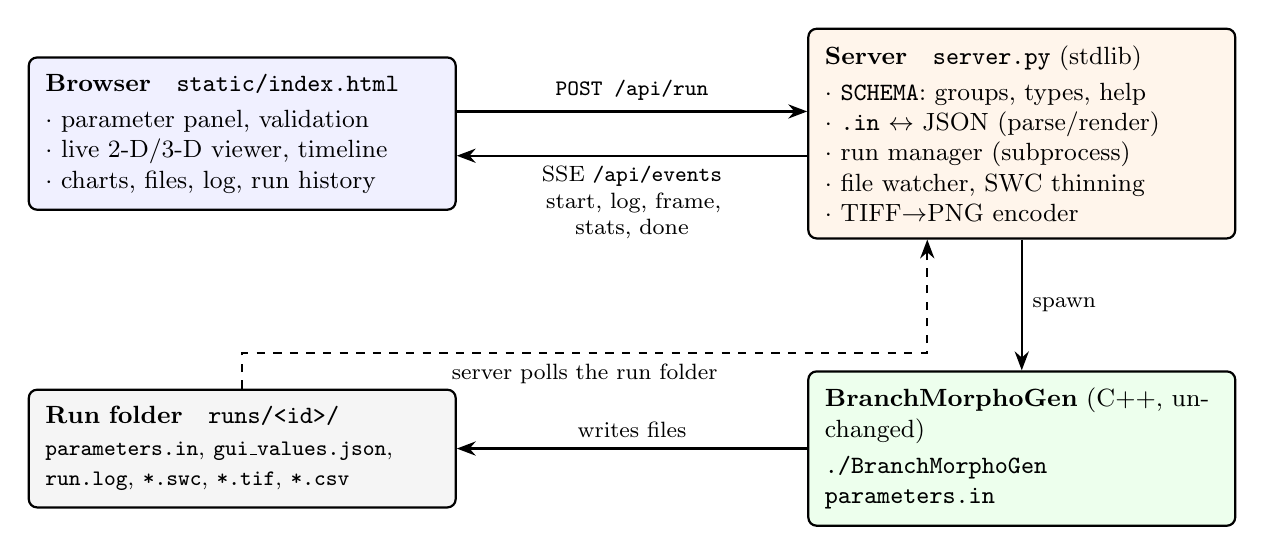
\begin{tikzpicture}[every node/.style={font=\small},
  box/.style={draw,rounded corners=3pt,thick,align=left,inner sep=6pt,fill=#1,text width=5.0cm},
  arr/.style={-{Stealth[length=2.4mm]},thick}, lab/.style={font=\footnotesize,fill=white,inner sep=1.5pt}]
  \node[box=blue!6] (br) at (0,0) {\textbf{Browser}\quad\code{static/index.html}\\[2pt]
     $\cdot$ parameter panel, validation\\ $\cdot$ live 2-D/3-D viewer, timeline\\ $\cdot$ charts, files, log, run history};
  \node[box=orange!8] (sv) at (9.9,0) {\textbf{Server}\quad\code{server.py} (stdlib)\\[2pt]
     $\cdot$ \code{SCHEMA}: groups, types, help\\ $\cdot$ \code{.in} $\leftrightarrow$ JSON (parse/render)\\ $\cdot$ run manager (subprocess)\\ $\cdot$ file watcher, SWC thinning\\ $\cdot$ TIFF$\to$PNG encoder};
  \node[box=green!7] (core) at (9.9,-4.0) {\textbf{BranchMorphoGen} (C++, unchanged)\\[2pt] \code{./BranchMorphoGen parameters.in}};
  \node[box=black!4] (fs) at (0,-4.0) {\textbf{Run folder}\quad\code{runs/<id>/}\\[2pt]
     {\footnotesize\mbox{\code{parameters.in}}, \mbox{\code{gui\_values.json}},\\ \code{run.log}, \code{*.swc}, \code{*.tif}, \code{*.csv}}};
  \draw[arr] ([yshift=8pt]br.east) -- node[lab,above=2pt]{\code{POST /api/run}} ([yshift=8pt]sv.west);
  \draw[arr] ([yshift=-8pt]sv.west) -- node[lab,below=2pt,align=center,text width=3.4cm]{SSE \code{/api/events}\\ start, log, frame,\\ stats, done} ([yshift=-8pt]br.east);
  \draw[arr] (sv.south) -- node[lab,right=2pt]{spawn} (core.north);
  \draw[arr] (core.west) -- node[lab,above=2pt]{writes files} (fs.east);
  \draw[arr,dashed] (fs.north) -- ++(0,0.45) -| node[lab,pos=0.25,below=2pt]{server polls the run folder} ([xshift=-1.2cm]sv.south);
\end{tikzpicture}}
\caption{\textbf{Architecture of the web GUI.} The browser sends the panel values. The server renders them into \code{parameters.in} in a new run folder and starts the unmodified simulator. It then polls the folder and streams each new frame, statistic and log line back to the browser over Server-Sent Events.}
\label{fig:gui}
\end{figure}

\subsection{Starting the GUI}
\begin{lstlisting}[language=bash]
mkdir -p build && cd build && cmake .. && make -j && cd ..   # build once
python3 webgui/server.py           # opens http://127.0.0.1:8050
\end{lstlisting}
Options:
\begin{itemize}
  \item \code{-{}-port N}: use a different port.
  \item \code{-{}-host 0.0.0.0}: listen on all interfaces.
  \item \code{-{}-binary PATH}: use a specific executable.
  \item \code{-{}-build}: build the core with CMake if no executable is found.
  \item \code{-{}-no-browser}: don't open a browser tab.
\end{itemize}
On a remote machine, keep the default host and forward the port: \code{ssh -L 8050:127.0.0.1:8050 user@host}.

\subsection{Features}
\begin{itemize}
  \item \textbf{Parameter panel.}
  \begin{itemize}
    \item Every key is listed, grouped as in \code{parameters.in}. Changed values are highlighted, and each key shows its description on hover.
    \item Time-dependent parameters are edited as \code{time : value} tables. Matrices are typed as \code{;}-separated rows.
    \item Values are checked as you type: the number of states must equal the number of velocities, and the matrices must be $n\times n$.
    \item An SWC file can be uploaded as the initial condition.
  \end{itemize}
  \item \textbf{Auto-run.} About one second after the last edit, the current run is stopped and a new one starts.
  \item \textbf{Fast preview.} The pixel size is raised to at least 2\,\textmu m and \code{N\_SWC} to at least 40, for the run only, so that frames arrive quickly. Turn it off for a run that uses exactly the panel values.
  \item \textbf{Viewer.}
  \begin{itemize}
    \item 2-D and 3-D views: zoom, pan, rotate, double-click to fit.
    \item Colour by path distance, branch order, radius or depth.
    \item The time-dependent boundary is drawn as a dashed box.
    \item The synthetic TIFF can be shown for each frame.
  \end{itemize}
  \item \textbf{Timeline.} Scrub, play and follow live; a sample selector appears for \code{NSample}$>1$. Charts show the numbers of tips and branches and the total length against time.
  \item \textbf{Files, log and runs.} Download the full-resolution SWC, TIFF and CSV files and the exact \code{parameters.in}. Read the simulator log. Replay any earlier run, or load its parameters back into the panel. Import or export \code{.in} files, and choose presets from the repository root.
\end{itemize}

\subsection{Implementation and development}
\paragraph{Server (\code{server.py}, $\sim$790 lines).}
\begin{itemize}
  \item \code{SCHEMA} lists every parameter: its group, its type and its help text. The types are \code{int}, \code{float}, \code{bool}, \code{choice}, \code{vec}, \code{matrix} and the time-dependent \code{timevec}, \code{timematrix} and \code{timescalar}. The front end builds its whole form from this list.
  \item \code{parse\_param\_text} and \code{render\_param\_text} convert between \code{.in} text and a dictionary. They copy the comment and \code{time:value} handling of \code{SimulationParameters.cpp}.
  \item \code{start\_run}/\code{stop\_run} create a timestamped run folder, write the file and manage the subprocess.
  \item \code{scan\_frames} and \code{read\_swc\_decimated} find new frames and thin each SWC to about 0.4\,\textmu m spacing before sending it, which keeps $10^6$-point trees fast to draw. Each frame is sent as JSON arrays \code{x,y,z,r,p} (\code{r} = radius, \code{p} = parent index).
  \item \code{tiff\_to\_png} converts the 16-bit TIFF to PNG in pure Python (\code{zlib}, \code{struct}), so Pillow is not needed.
  \item \code{\_events} is the SSE loop. It sends \code{start}, \code{log}, \code{frame}, \code{stats} and \code{done} events.
\end{itemize}

\paragraph{Front end (\code{static/index.html}, $\sim$720 lines).}
A single page with no framework:
\begin{itemize}
  \item Branch order and path distance are computed in the browser from the parent array in one pass.
  \item Drawing uses an HTML canvas, in both 2-D and 3-D.
\end{itemize}

\paragraph{Extending the GUI.}
\begin{enumerate}
  \item \textbf{New parameter.} Add the key to the C++ parser (\code{SimulationParameters.h/.cpp}), then add one line to \code{SCHEMA}. The panel, validation, import and export pick it up automatically.
  \item \textbf{New colour mode or chart.} Edit \code{index.html}; all the data needed is already in the frame JSON.
  \item \textbf{New output file type.} Add its pattern to \code{scan\_frames} and the \code{/files/} handler.
\end{enumerate}

%=====================================================================
\section{Troubleshooting}
%=====================================================================
\begin{center}\small
\begin{tabularx}{\textwidth}{@{}p{5.2cm}X@{}}
\toprule
\textbf{Symptom} & \textbf{Fix}\\ \midrule
\code{TIFF library not found} & Install libtiff or set \code{TIFF\_ROOT} / \code{-DTIFF\_ROOT}.\\
Build fails & Check \code{build/CMakeFiles/CMakeError.log}; make sure the compiler supports C++17.\\
\code{Warning: Unknown key} & The key is misspelled or uses an old name; it is ignored.\\
\code{Mixed time-based and constant values} & Use either a constant or a \code{t:value} table for one parameter, not both.\\
\code{No .swc files found} & Check \code{SWCFileName} (file or folder).\\
Slow runs & A large $\lVert\mathbf K\rVert\Delta t$ is inaccurate, and a small $\Delta t$ or $\Delta s$ is slow. Use a coarser \code{pixelsize} while exploring.\\
Tips stuck at the soma or boundary & Check \code{RadiusSoma} against \code{InitialLength}, and the box limits at \code{Time\_Start}.\\
GUI: binary not found / port in use & Use \code{-{}-build} or \code{--binary}; or use \code{--port}.\\
\bottomrule
\end{tabularx}
\end{center}

%=====================================================================
\section*{How to cite}
%=====================================================================
\addcontentsline{toc}{section}{How to cite}
If you use BranchMorphoGen, please cite the software (\code{Citation.cff}) and S.~Sutradhar, S.~Shree and J.~Howard, \emph{BranchMorphoGen: a generalized framework to simulate branching morphogenesis} (in preparation), together with Refs.~\cite{Shree2022,Ouyang2025} for the underlying tip dynamics.

%=====================================================================
\section*{Acknowledgements}
%=====================================================================
\addcontentsline{toc}{section}{Acknowledgements}
BranchMorphoGen was developed in the Howard Lab at Yale University. The scientific model, the C++ simulation core, the parameter values and all figures are the work of the authors.

\paragraph{Use of AI tools.} The web graphical interface (\code{webgui/}: \code{server.py}, \code{static/index.html} and its README) and this user manual were written with the help of \textbf{Claude} (Anthropic), using Claude Code. The authors reviewed and verified the generated code and text.

% Bibliography is embedded so the document compiles with plain pdflatex
% (no BibTeX run needed). It was generated from references.bib with unsrtnat.
% To regenerate after editing references.bib: replace this block with
%   \bibliographystyle{unsrtnat}\bibliography{references}
% and build with: latexmk -pdf BranchMorphoGen_UserManual.tex
\begin{thebibliography}{20}
\providecommand{\natexlab}[1]{#1}
\providecommand{\url}[1]{\texttt{#1}}
\expandafter\ifx\csname urlstyle\endcsname\relax
  \providecommand{\doi}[1]{doi: #1}\else
  \providecommand{\doi}{doi: \begingroup \urlstyle{rm}\Url}\fi

\bibitem[Hannezo et~al.(2017)Hannezo, Scheele, Moad, Drogo, Harnett, Cho, and
  Klein]{Hannezo2017}
E~Hannezo, C~L~M Scheele, M~Moad, G~Drogo, M~R Harnett, M~J Cho, and A~M Klein.
\newblock A unifying theory of branching morphogenesis.
\newblock \emph{Cell}, 171:\penalty0 242--255, 2017.

\bibitem[Uçar et~al.(2021)Uçar, Kamenev, Sunadome, Fachet, Lallemend,
  Adameyko, Hadjab, and Hannezo]{Uar2021}
Mehmet~Can Uçar, Dmitrii Kamenev, Kazunori Sunadome, Dominik Fachet, Francois
  Lallemend, Igor Adameyko, Saida Hadjab, and Edouard Hannezo.
\newblock Theory of branching morphogenesis by local interactions and global
  guidance.
\newblock \emph{Nature Communications}, 12, 12 2021.
\newblock ISSN 20411723.
\newblock \doi{10.1038/s41467-021-27135-5}.

\bibitem[Cuntz et~al.(2010)Cuntz, Forstner, Borst, and H{\"a}usser]{Cuntz2010}
Hermann Cuntz, Friedrich Forstner, Alexander Borst, and Michael H{\"a}usser.
\newblock One rule to grow them all: A general theory of neuronal branching and
  its practical application.
\newblock \emph{PLoS Computational Biology}, 6\penalty0 (8):\penalty0 e1000877,
  2010.

\bibitem[Koene et~al.(2009)Koene, Tijms, Hees, Postma, Ridder, Ramakers, Pelt,
  and Ooyen]{Koene2009}
Randal~A. Koene, Betty Tijms, Peter~Van Hees, Frank Postma, Alexander~De
  Ridder, Ger~J.A. Ramakers, Jaap~Van Pelt, and Arjen~Van Ooyen.
\newblock Netmorph: A framework for the stochastic generation of large scale
  neuronal networks with realistic neuron morphologies.
\newblock \emph{Neuroinformatics}, 7:\penalty0 195--210, 9 2009.
\newblock ISSN 15392791.
\newblock \doi{10.1007/s12021-009-9052-3}.

\bibitem[Palavalli et~al.(2021)Palavalli, Tizón-Escamilla, Rupprecht, and
  Lecuit]{Palavalli2021}
Amrutha Palavalli, Nicolás Tizón-Escamilla, Jean~François Rupprecht, and
  Thomas Lecuit.
\newblock Deterministic and stochastic rules of branching govern dendrite
  morphogenesis of sensory neurons.
\newblock \emph{Current Biology}, 31:\penalty0 459--472.e4, 2 2021.
\newblock ISSN 18790445.
\newblock \doi{10.1016/j.cub.2020.10.054}.

\bibitem[Castro et~al.(2020)Castro, Baltruschat, Stürner, Bahrami, Jedlicka,
  Tavosanis, and Cuntz]{Castro2020}
André~Ferreira Castro, Lothar Baltruschat, Tomke Stürner, Amirhoushang
  Bahrami, Peter Jedlicka, Gaia Tavosanis, and Hermann Cuntz.
\newblock Achieving functional neuronal dendrite structure through sequential
  stochastic growth and retraction.
\newblock \emph{eLife}, 9:\penalty0 1--38, 10 2020.
\newblock ISSN 2050084X.
\newblock \doi{10.7554/eLife.60920}.

\bibitem[Ganguly et~al.(2016)Ganguly, Trottier, Liang, Bowne-Anderson, and
  Howard]{Ganguly2016}
Sujoy Ganguly, Olivier Trottier, Xin Liang, Hugo Bowne-Anderson, and Jonathon
  Howard.
\newblock Morphology of fly larval class {IV} dendrites accords with a random
  branching and contact based branch deletion model.
\newblock \emph{arXiv preprint arXiv:1611.05918}, 2016.

\bibitem[Shree et~al.(2022)Shree, Sutradhar, Trottier, Tu, Liang, and
  Howard]{Shree2022}
Sonal Shree, Sabyasachi Sutradhar, Olivier Trottier, Yuhai Tu, Xin Liang, and
  Jonathon Howard.
\newblock Dynamic instability of dendrite tips generates the highly branched
  morphologies of sensory neurons.
\newblock \emph{Science Advances}, 8:\penalty0 eabn0080, 2022.

\bibitem[Ouyang et~al.(2025)Ouyang, Sutradhar, Trottier, Shree, Yu, Tu, and
  Howard]{Ouyang2025}
Xiaoyi Ouyang, Sabyasachi Sutradhar, Olivier Trottier, Sonal Shree, Qiwei Yu,
  Yuhai Tu, and Jonathon Howard.
\newblock Neurons exploit stochastic growth to rapidly and economically build
  dense dendritic arbors.
\newblock \emph{Nature Communications}, 16, 12 2025.
\newblock ISSN 20411723.
\newblock \doi{10.1038/s41467-025-60800-7}.

\bibitem[Dogterom and Leibler(1993)]{Dogterom1993}
Marileen Dogterom and Stanislas Leibler.
\newblock Physical aspects of the growth and regulation of microtubule
  structures.
\newblock \emph{Physical Review Letters}, 70\penalty0 (9):\penalty0 1347--1350,
  1993.

\bibitem[Gillespie(1977)]{Gillespie1977}
Daniel~T. Gillespie.
\newblock Exact stochastic simulation of coupled chemical reactions.
\newblock \emph{The Journal of Physical Chemistry}, 81\penalty0 (25):\penalty0
  2340--2361, 1977.

\bibitem[Matthews et~al.(2007)Matthews, Kim, Flanagan, Hattori, Clemens,
  Zipursky, and Grueber]{Matthews2007}
Benjamin~J. Matthews, Michelle~E. Kim, John~J. Flanagan, Daisuke Hattori,
  James~C. Clemens, S.~ Lawrence Zipursky, and Wesley~B. Grueber.
\newblock Dendrite self-avoidance is controlled by dscam.
\newblock \emph{Cell}, 129:\penalty0 593--604, 5 2007.
\newblock ISSN 00928674.
\newblock \doi{10.1016/j.cell.2007.04.013}.

\bibitem[Rall(1959)]{Rall1959}
Wilfrid Rall.
\newblock Branching dendritic trees and motoneuron membrane resistivity.
\newblock \emph{Experimental Neurology}, 1\penalty0 (5):\penalty0 491--527,
  1959.

\bibitem[Murray(1926)]{Murray1926}
Cecil~D. Murray.
\newblock The physiological principle of minimum work: {I}. {T}he vascular
  system and the cost of blood volume.
\newblock \emph{Proceedings of the National Academy of Sciences USA},
  12\penalty0 (3):\penalty0 207--214, 1926.

\bibitem[Dikec et~al.(2020)Dikec, Olivier, Bobée, D'Angelo, Catellier, David,
  Filaine, Herbert, Lalanne, Lalucque, Monasse, Rieu, Ruprich-Robert, Véber,
  Chapeland-Leclerc, and Herbert]{Dikec2020}
J.~Dikec, A.~Olivier, C.~Bobée, Y.~D'Angelo, R.~Catellier, P.~David,
  F.~Filaine, S.~Herbert, Ch~Lalanne, H.~Lalucque, L.~Monasse, M.~Rieu,
  G.~Ruprich-Robert, A.~Véber, F.~Chapeland-Leclerc, and E.~Herbert.
\newblock Hyphal network whole field imaging allows for accurate estimation of
  anastomosis rates and branching dynamics of the filamentous fungus podospora
  anserina.
\newblock \emph{Scientific reports}, 10:\penalty0 3131, 2 2020.
\newblock ISSN 20452322.
\newblock \doi{10.1038/s41598-020-57808-y}.

\bibitem[Ledoux et~al.(2022)Ledoux, Chapeland-Leclerc, Ruprich-Robert, Bobée,
  Lalanne, Éric Herbert, and David]{Ledoux2022}
Clara Ledoux, Florence Chapeland-Leclerc, Gwenaël Ruprich-Robert, Cécilia
  Bobée, Christophe Lalanne, Éric Herbert, and Pascal David.
\newblock Prediction and experimental evidence of the optimisation of the
  angular branching process in the thallus growth of podospora anserina.
\newblock \emph{Scientific Reports}, 12, 12 2022.
\newblock ISSN 20452322.
\newblock \doi{10.1038/s41598-022-16245-9}.

\bibitem[Honda(1971)]{Honda1971}
Hisao Honda.
\newblock Description of the form of trees by the parameters of the tree-like
  body: Effects of the branching angle and the branch length on the shape of
  the tree-like body.
\newblock \emph{J. theor. Biol}, 31:\penalty0 331--338, 1971.

\bibitem[Ascoli et~al.(2007)Ascoli, Donohue, and Halavi]{Ascoli2007}
Giorgio~A. Ascoli, Duncan~E. Donohue, and Maryam Halavi.
\newblock Neuromorpho.org: A central resource for neuronal morphologies.
\newblock \emph{Journal of Neuroscience}, 27:\penalty0 9247--9251, 8 2007.
\newblock ISSN 02706474.
\newblock \doi{10.1523/JNEUROSCI.2055-07.2007}.

\bibitem[Kanari et~al.(2018)Kanari, Dłotko, Scolamiero, Levi, Shillcock, Hess,
  and Markram]{Kanari2018}
Lida Kanari, Paweł Dłotko, Martina Scolamiero, Ran Levi, Julian Shillcock,
  Kathryn Hess, and Henry Markram.
\newblock A topological representation of branching neuronal morphologies.
\newblock \emph{Neuroinformatics}, 16:\penalty0 3--13, 1 2018.
\newblock ISSN 15392791.
\newblock \doi{10.1007/s12021-017-9341-1}.

\bibitem[Liao et~al.(2023)Liao, Bird, Cuntz, and Howard]{Liao2023}
Maijia Liao, Alex~D. Bird, Hermann Cuntz, and Jonathon Howard.
\newblock Topology recapitulates morphogenesis of neuronal dendrites.
\newblock \emph{Cell Reports}, 42, 11 2023.
\newblock ISSN 22111247.
\newblock \doi{10.1016/j.celrep.2023.113268}.

\end{thebibliography}

\end{document}
